\section{Shape of the aggregation estimators}\label{FREQ_GENERAL_SHAPE}\label{freq:ge:shape}

We want to define a family of estimators $(\widehat{\theta}^{(\eta)})_{\eta \in ]0, \infty]}$ of $\theta^{\circ}$ and estimators for $f$, $\widehat{f}^{(\eta)} := \fourier^{\star}(\widehat{\theta}^{(\eta)})$ such that, for any $\eta$, $\widehat{\theta}^{(\eta)}$ has the shape
\begin{equation}\label{freq:ge:shape:kn}
(\widehat{\theta}^{(\eta)}(s))_{s \in \mathds{F}} = \sum\nolimits_{m \in \N} \P_{M}^{(\eta)}(m) \cdot (\theta_{n, \overline{m}}(s))_{s \in \mathds{F}} = \sum\nolimits_{m \geq \vert s \vert} \P_{M}^{(\eta)}(m) \cdot (\theta_{n}(s))_{s \in \mathds{F}}
\end{equation}
under \nref{AS_INTRO_DATA_KNOWN}, and
\begin{equation}\label{freq:ge:shape:uk}
(\widehat{\theta}^{(\eta)}(s))_{s \in \mathds{F}} = \sum\nolimits_{m \in \N} \widehat{\P}_{M}^{(\eta)}(m) \cdot (\theta_{n, n_{\lambda}, \overline{m}}(s))_{s \in \mathds{F}} = \sum\nolimits_{m \geq \vert s \vert} \widehat{\P}_{M}^{(\eta)}(m) \cdot (\theta_{n, n_{\lambda}}(s))_{s \in \mathds{F}}
\end{equation}
under \nref{AS_INTRO_DATA_UNKNOWN}.
The sequence $(\P_{M}^{(\eta)}(m))_{m \in \N}$ is the aggregation sequence.
Under \nref{AS_INTRO_DATA_KNOWN} it depends on the observations $Y^{n}$ as well on the known operator $T$ through its eigen values $(\lambda(s))_{s \in \mathds{F}}$ whereas under \nref{AS_INTRO_DATA_UNKNOWN}, it only depends on the observed data $Y^{n}$ and $\epsilon^{n_{\lambda}}$.
This notation is motivated by the Bayesian inspiration of the method.

We give in \nref{fig:ge:adaptive:aggregation} an illustration of the aggregation estimator used in a Gaussian sequence space model in the direct problem case, that is to say $\lambda(s) = 1$ for any $s$ in $\N$.

\begin{figure}
  \centering
  \begin{tabular}{@{}c@{}}
    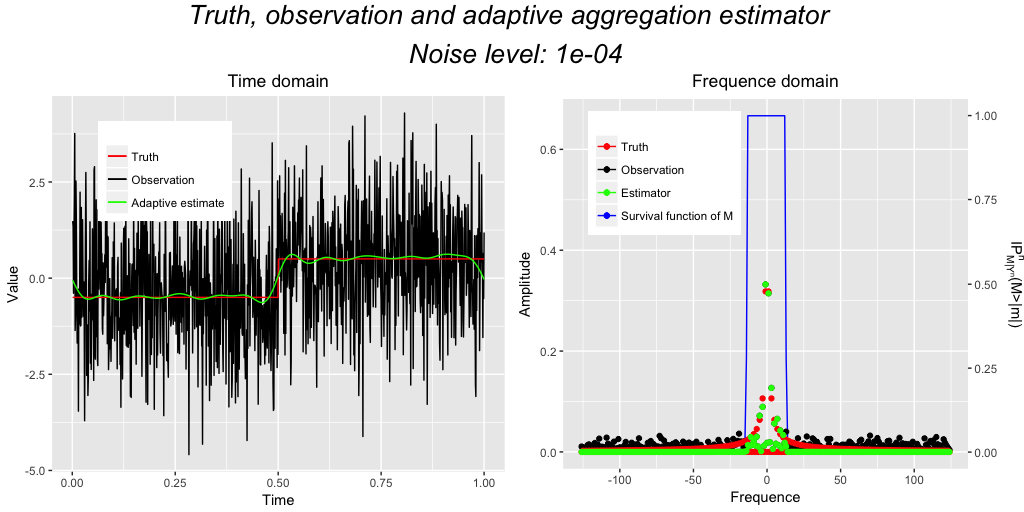
\includegraphics[width=.49\linewidth]{gauss/adaptive/aggregation_surv.png} \\[\abovecaptionskip]
  \end{tabular}
  \begin{tabular}{@{}c@{}}
    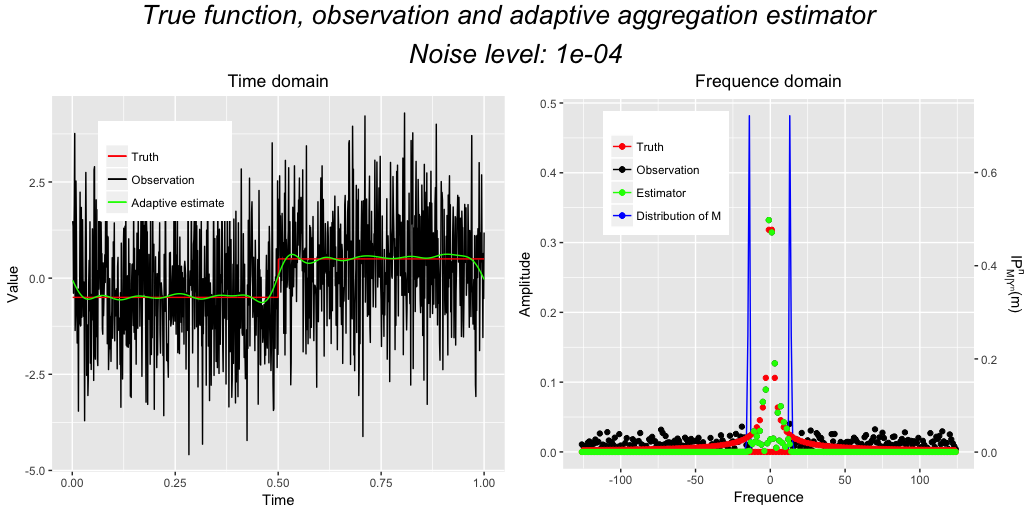
\includegraphics[width=.49\linewidth]{gauss/adaptive/aggregation.png} \\[\abovecaptionskip]
  \end{tabular}
  \caption{Aggregation estimator on an Gaussian sequence space model, direct problem case}
  \label{fig:ge:adaptive:aggregation}
\end{figure}

Taking inspiration in the posterior distributions obtained with a hierarchical prior in the previous chapter, we will give the following shape to the aggregation weights.
In the case \nref{AS_INTRO_DATA_KNOWN} let be the following functions
\begin{multline}\label{freq:ge:shape:kn:we}
\Upsilon : \mathds{N} \to \R_{+}, \quad m \mapsto \Upsilon(m); \qquad \pen^{\Lambda} : \N \to \R_{+}, \quad m \mapsto \pen^{\Lambda}(m);\\
\P_{M}^{(\eta)} : \N \to \R_{+}, \quad m \mapsto \tfrac{\exp[-\eta n (-\Upsilon(m) + \pen^{\Lambda}(m))]}{\sum\nolimits_{k = 0}^{n} \exp[-\eta n (-\Upsilon(k) + \pen^{\Lambda}(k))]} \mathds{1}_{m \leq n};
\end{multline}
where $\Upsilon$ depends on the observations $Y^{n}$ as well as the known operator $T$ through the sequence $\lambda$ of its eigen values; and $\pen^{\Lambda}$ depends only on the parameter $T$ through the sequence $\lambda$ of its eigen values.
Under \nref{AS_INTRO_DATA_UNKNOWN}, we define
\begin{multline}\label{freq:ge:shape:uk:we}
\Upsilon : \N \to \R_{+}, \quad m \mapsto \Upsilon(m); \qquad \pen^{\widehat{\Lambda}} : \N \to \R_{+}, \quad m \mapsto \pen^{\widehat{\Lambda}}(m);\\
\widehat{\P}_{M}^{(\eta)} : \N \to \R_{+}; \quad m \mapsto \tfrac{\exp[\eta n (\Upsilon(m) - \pen^{\widehat{\Lambda}}(m))]}{\sum\nolimits_{k = 0}^{n} \exp[\eta n (\Upsilon(k) - \pen^{\widehat{\Lambda}}(k))]} \mathds{1}_{m \leq n};
\end{multline}
where $\Upsilon$ depends solely the observations $Y^{n}$ and $\epsilon^{n_{\lambda}}$; and $\pen^{\widehat{\Lambda}}$ depends only on the observations $\epsilon^{n_{\lambda}}$.
The functions $\Upsilon$, and $\pen^{\Lambda}$ will respectively be called contrast and penalty.
For any subset $S$ of $\N$, we denote $\P_{M}^{(\eta)}(S) = \sum_{k \in S} \P_{M}^{(\eta)}(k)$.
One would expect that as the amount of data increases, the number of coefficients estimated increases too, as our observations allows us to recover more information about the system of interest as illustrated in \nref{fig:ge:adaptive:M} by representing $\P_{M}^{(\eta)}(\llbracket m, n \rrbracket)$ for increasnig values of $n$.

\begin{figure}
  \centering
  \begin{tabular}{@{}c@{}}
    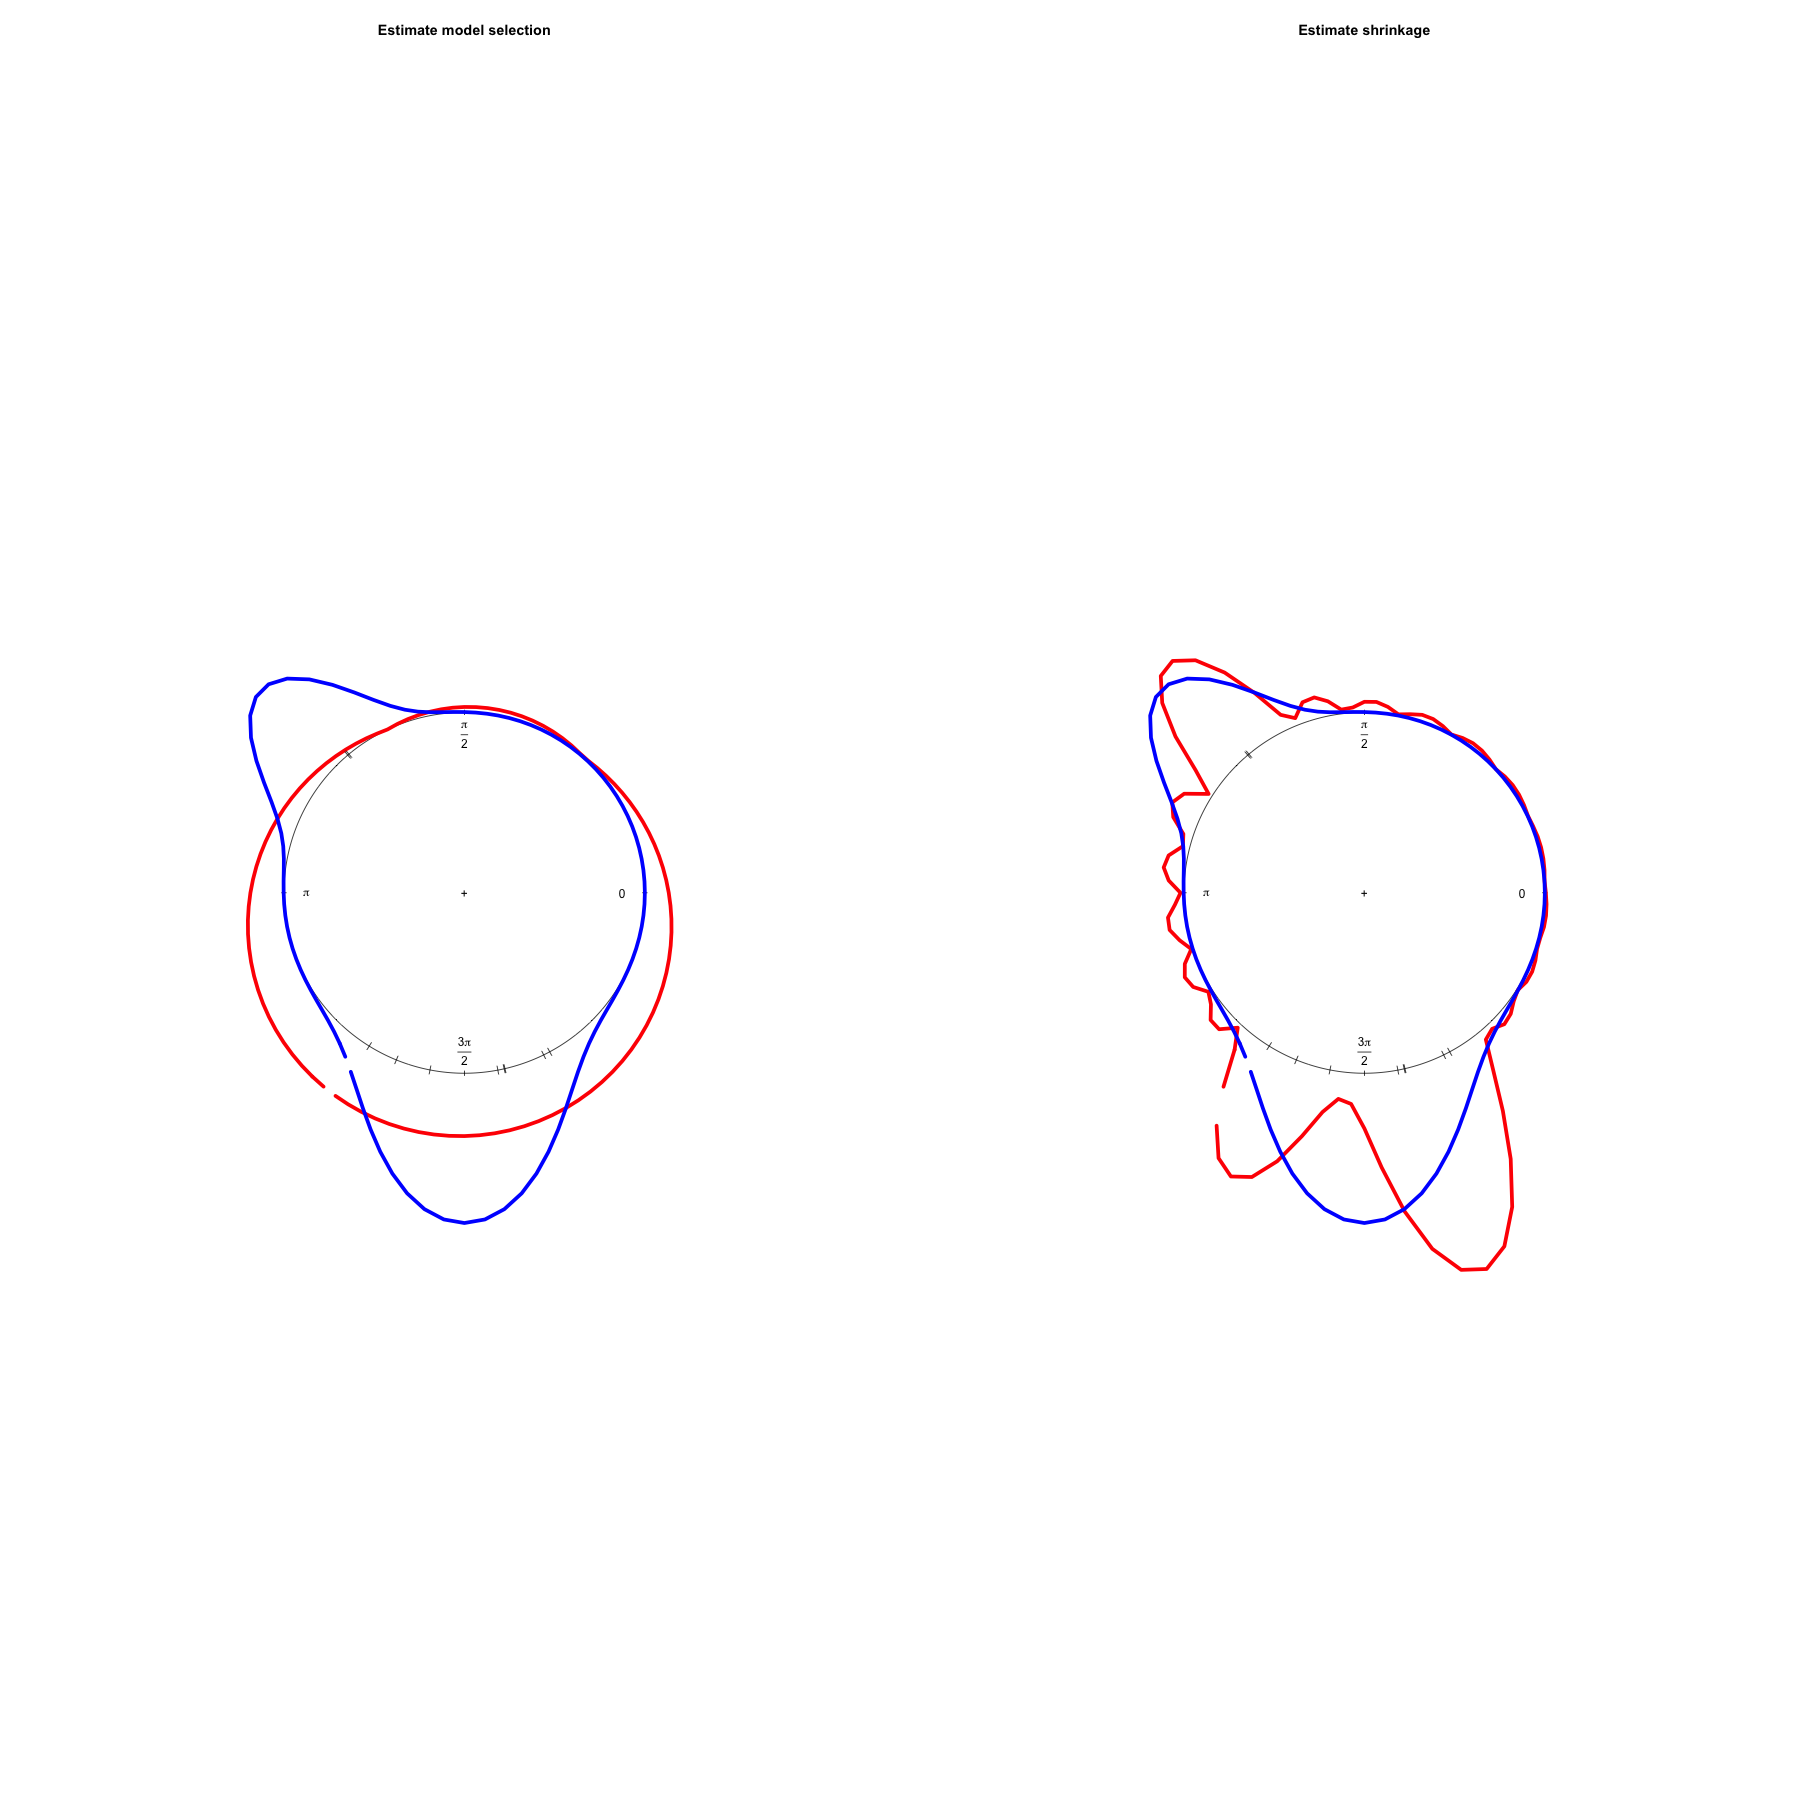
\includegraphics[width=.49\linewidth]{density/distM/1.png} \\[\abovecaptionskip]
  \end{tabular}
  \begin{tabular}{@{}c@{}}
    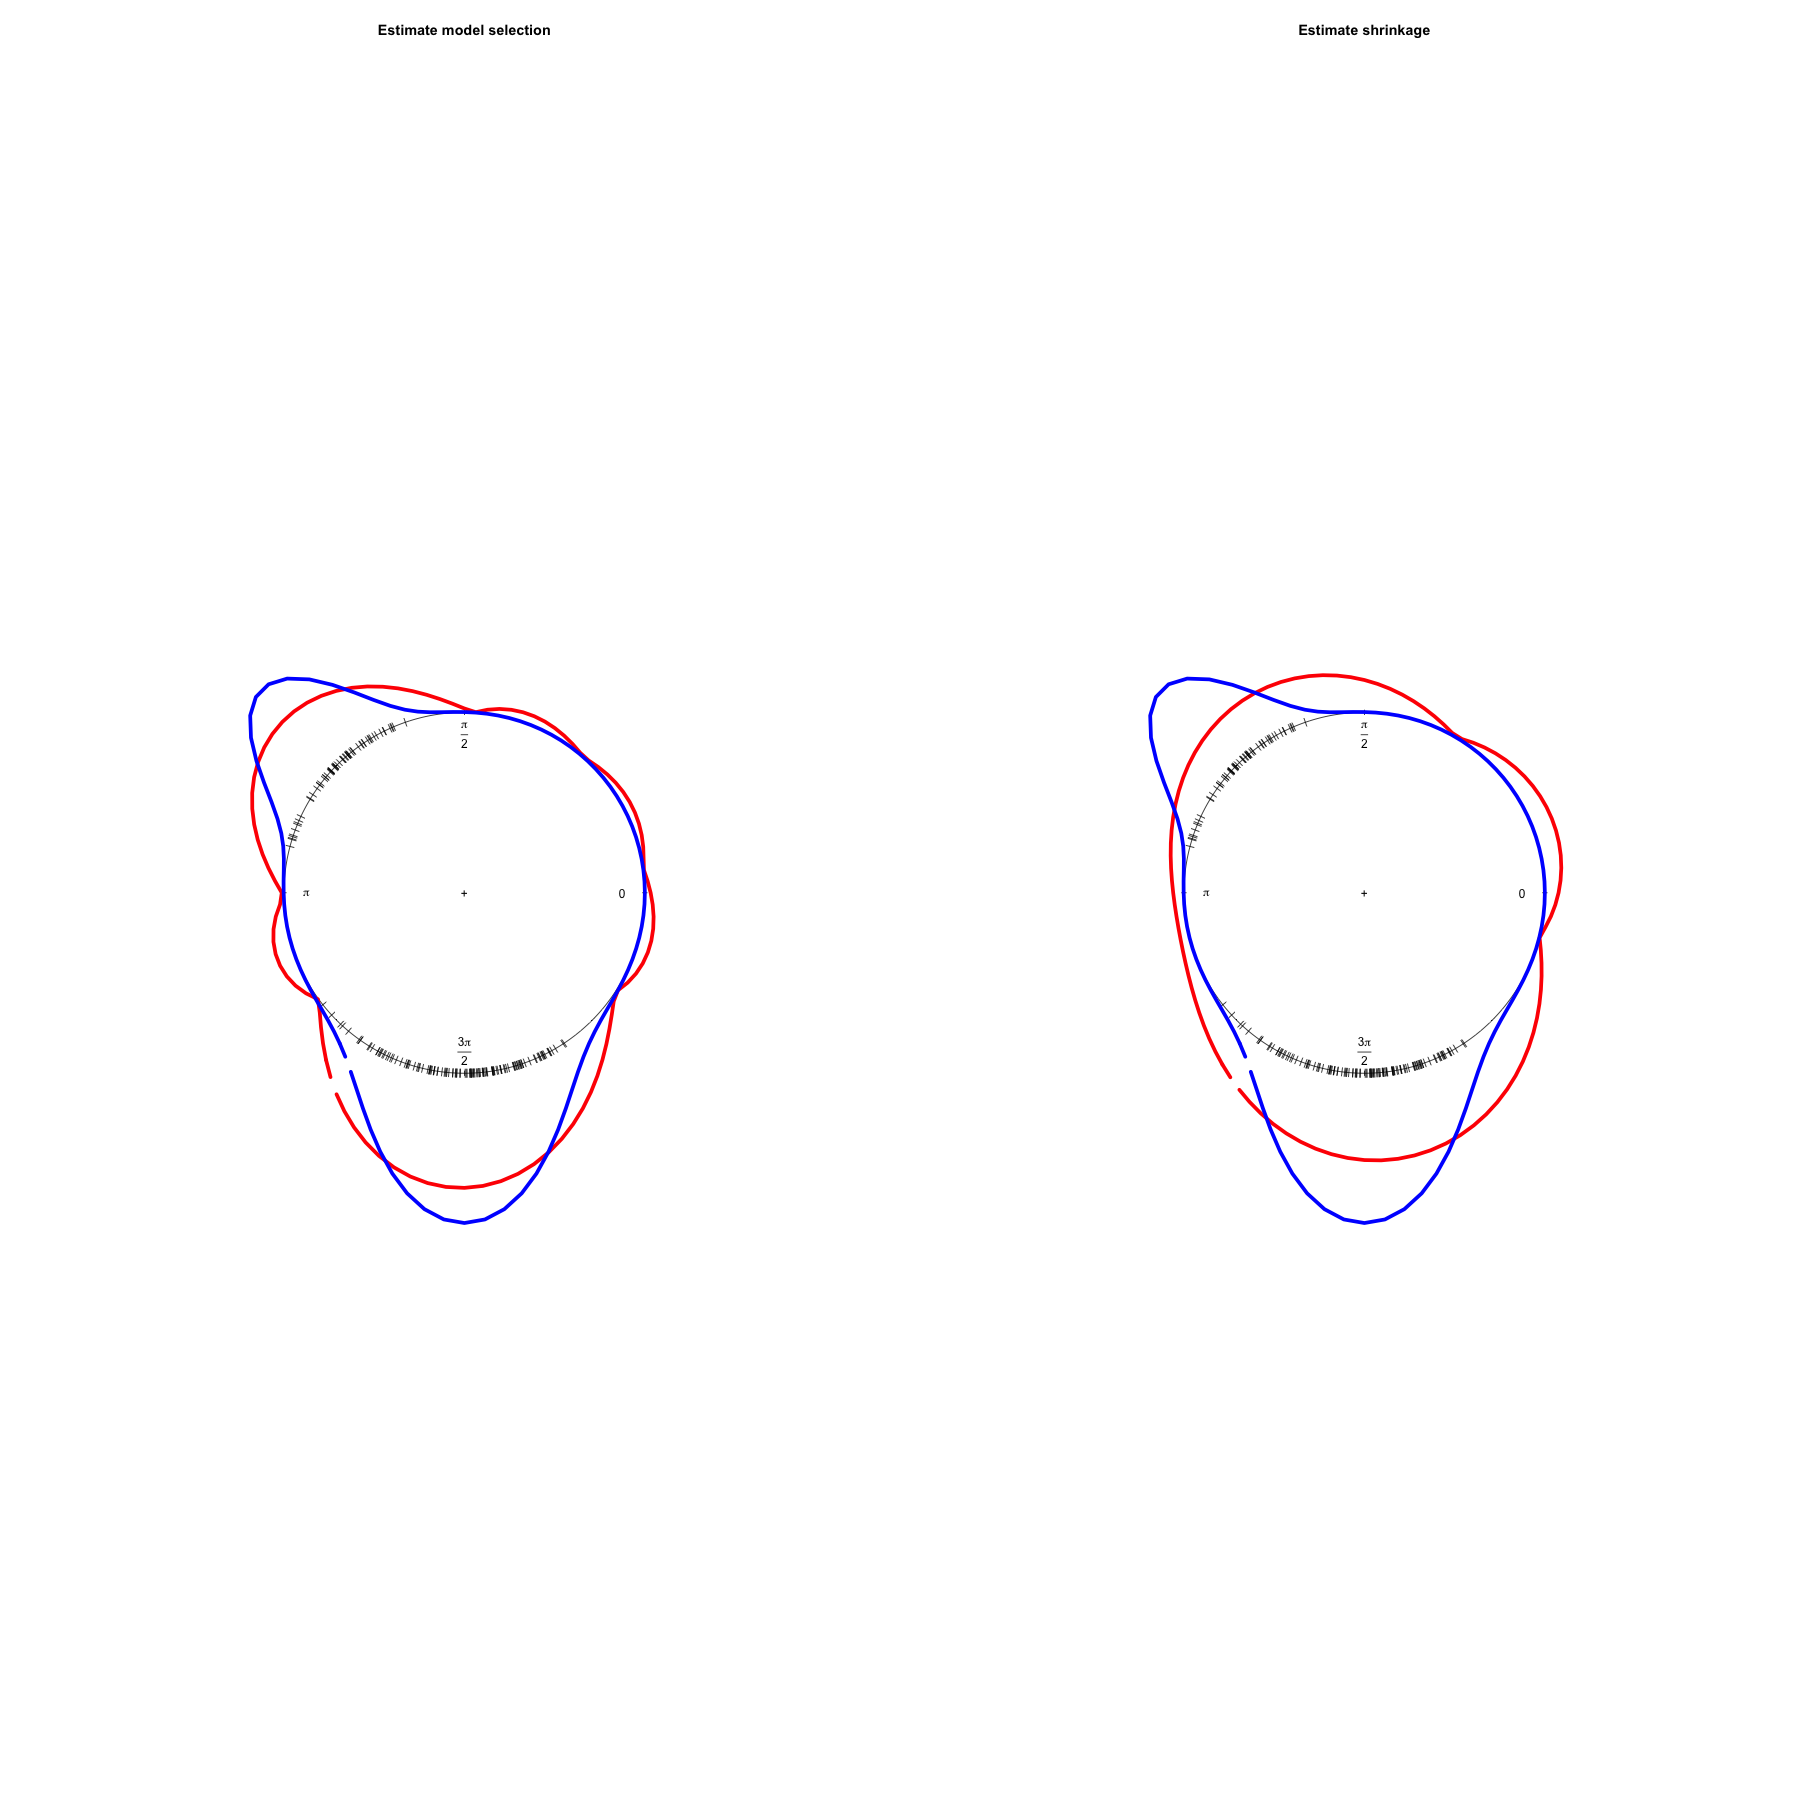
\includegraphics[width=.49\linewidth]{density/distM/20.png} \\[\abovecaptionskip]
  \end{tabular}
  
    \begin{tabular}{@{}c@{}}
    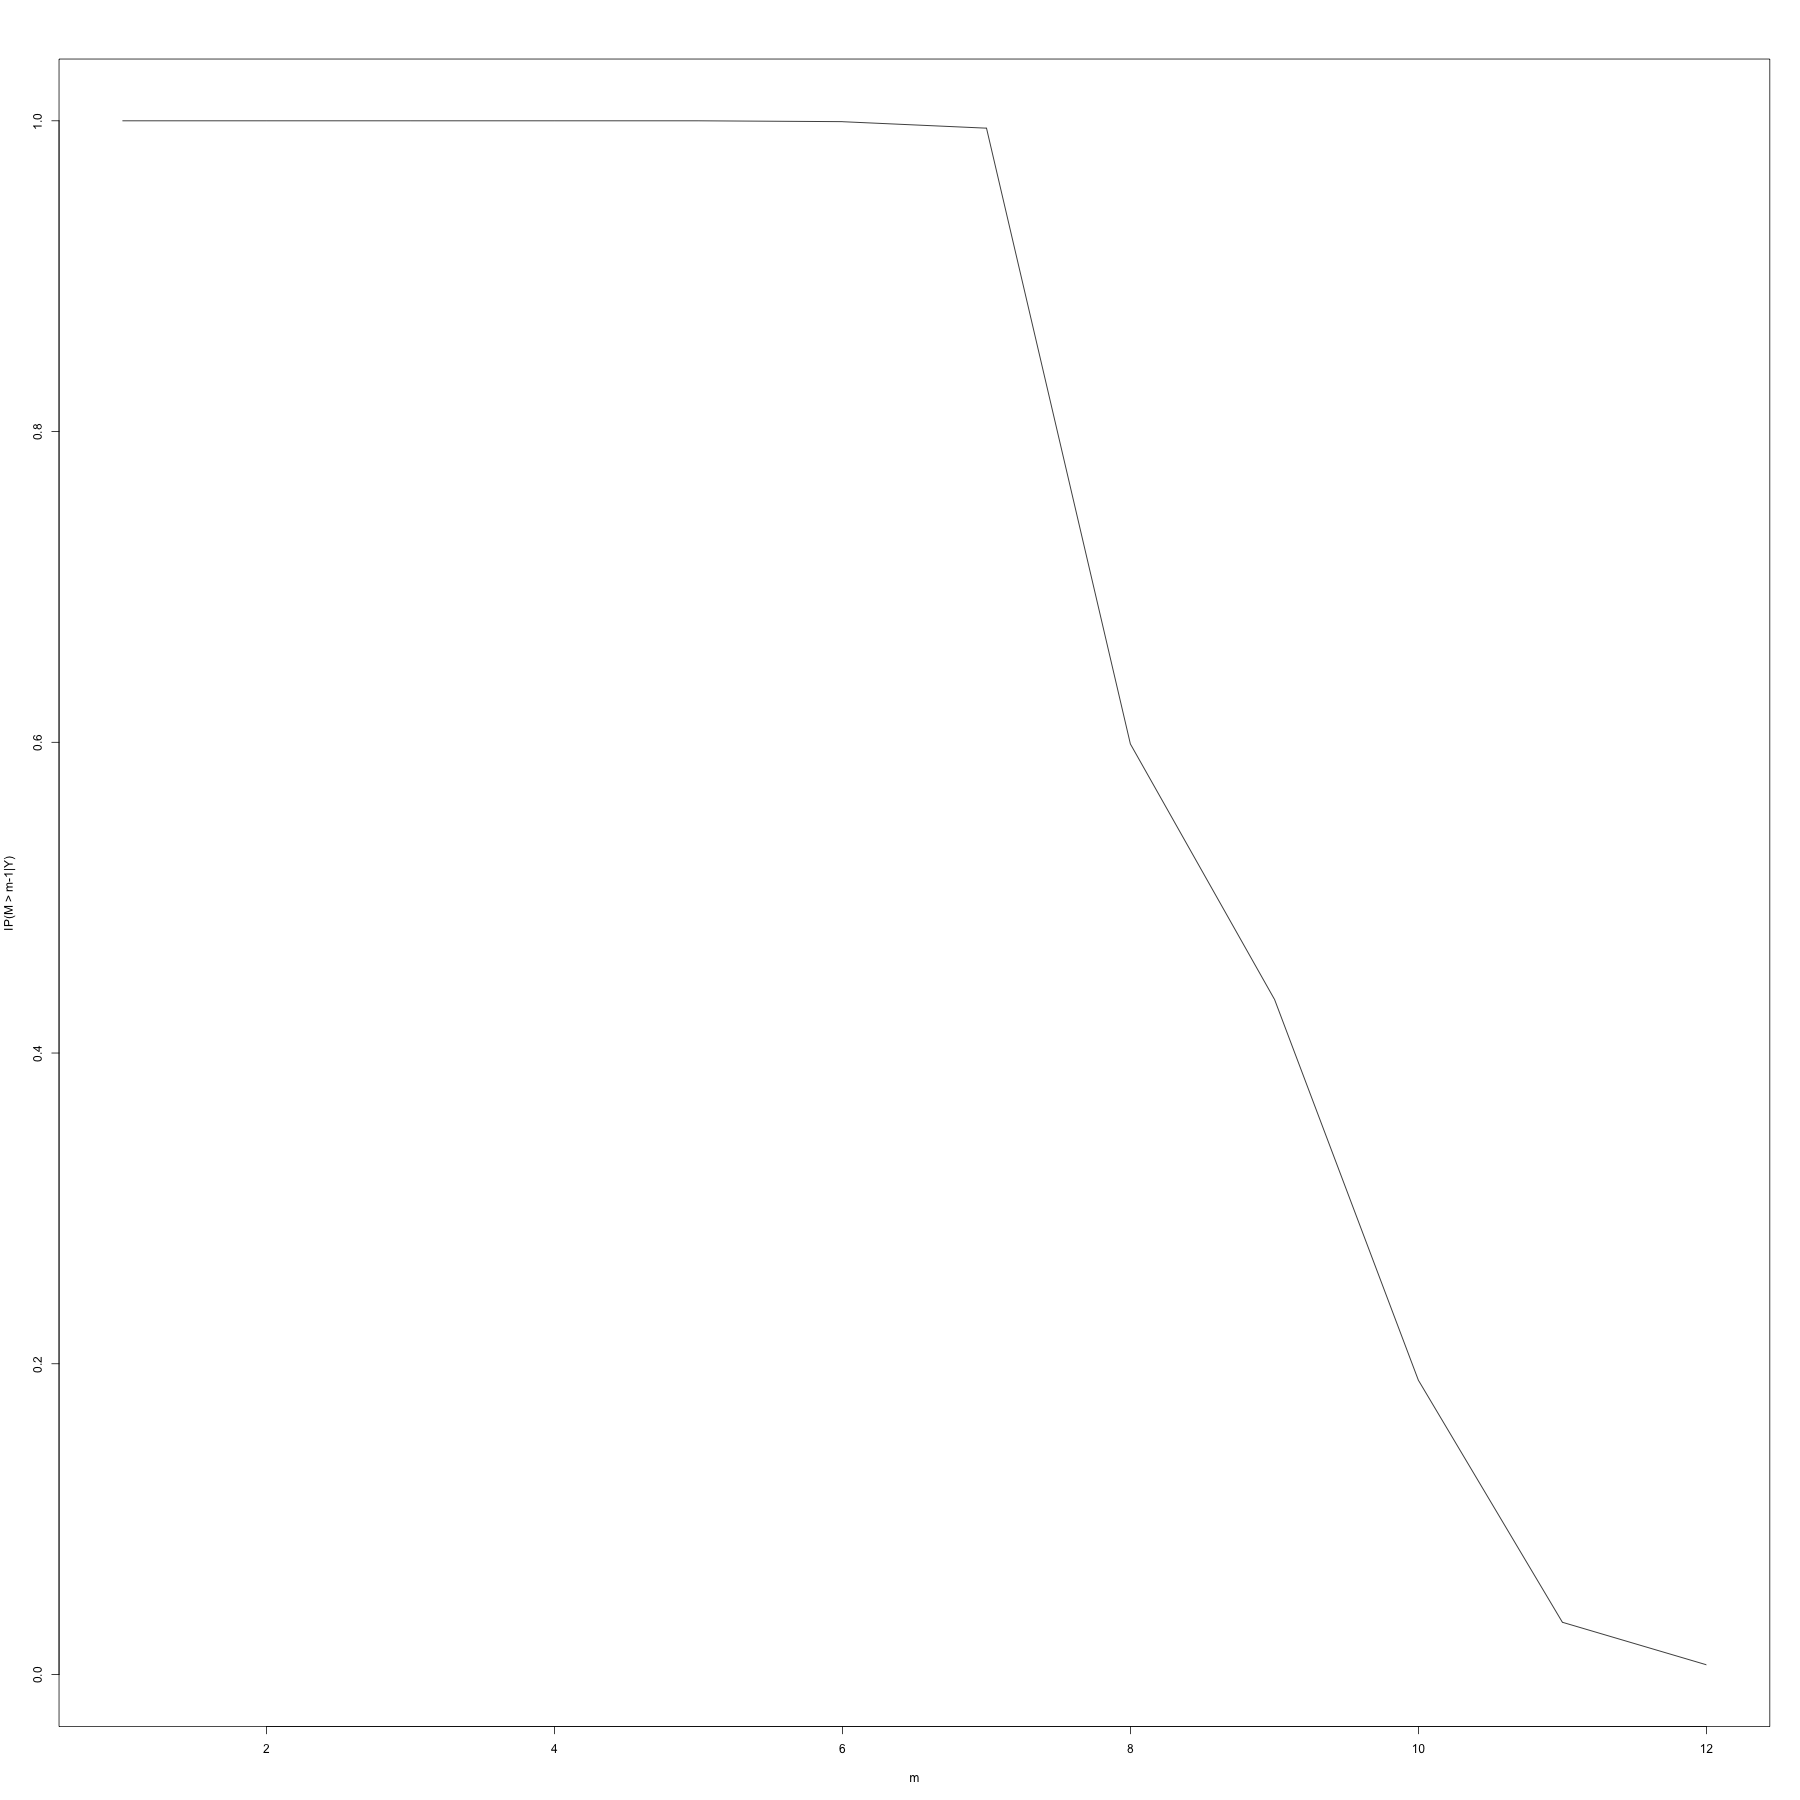
\includegraphics[width=.49\linewidth]{density/distM/40.png} \\[\abovecaptionskip]
  \end{tabular}
  \begin{tabular}{@{}c@{}}
    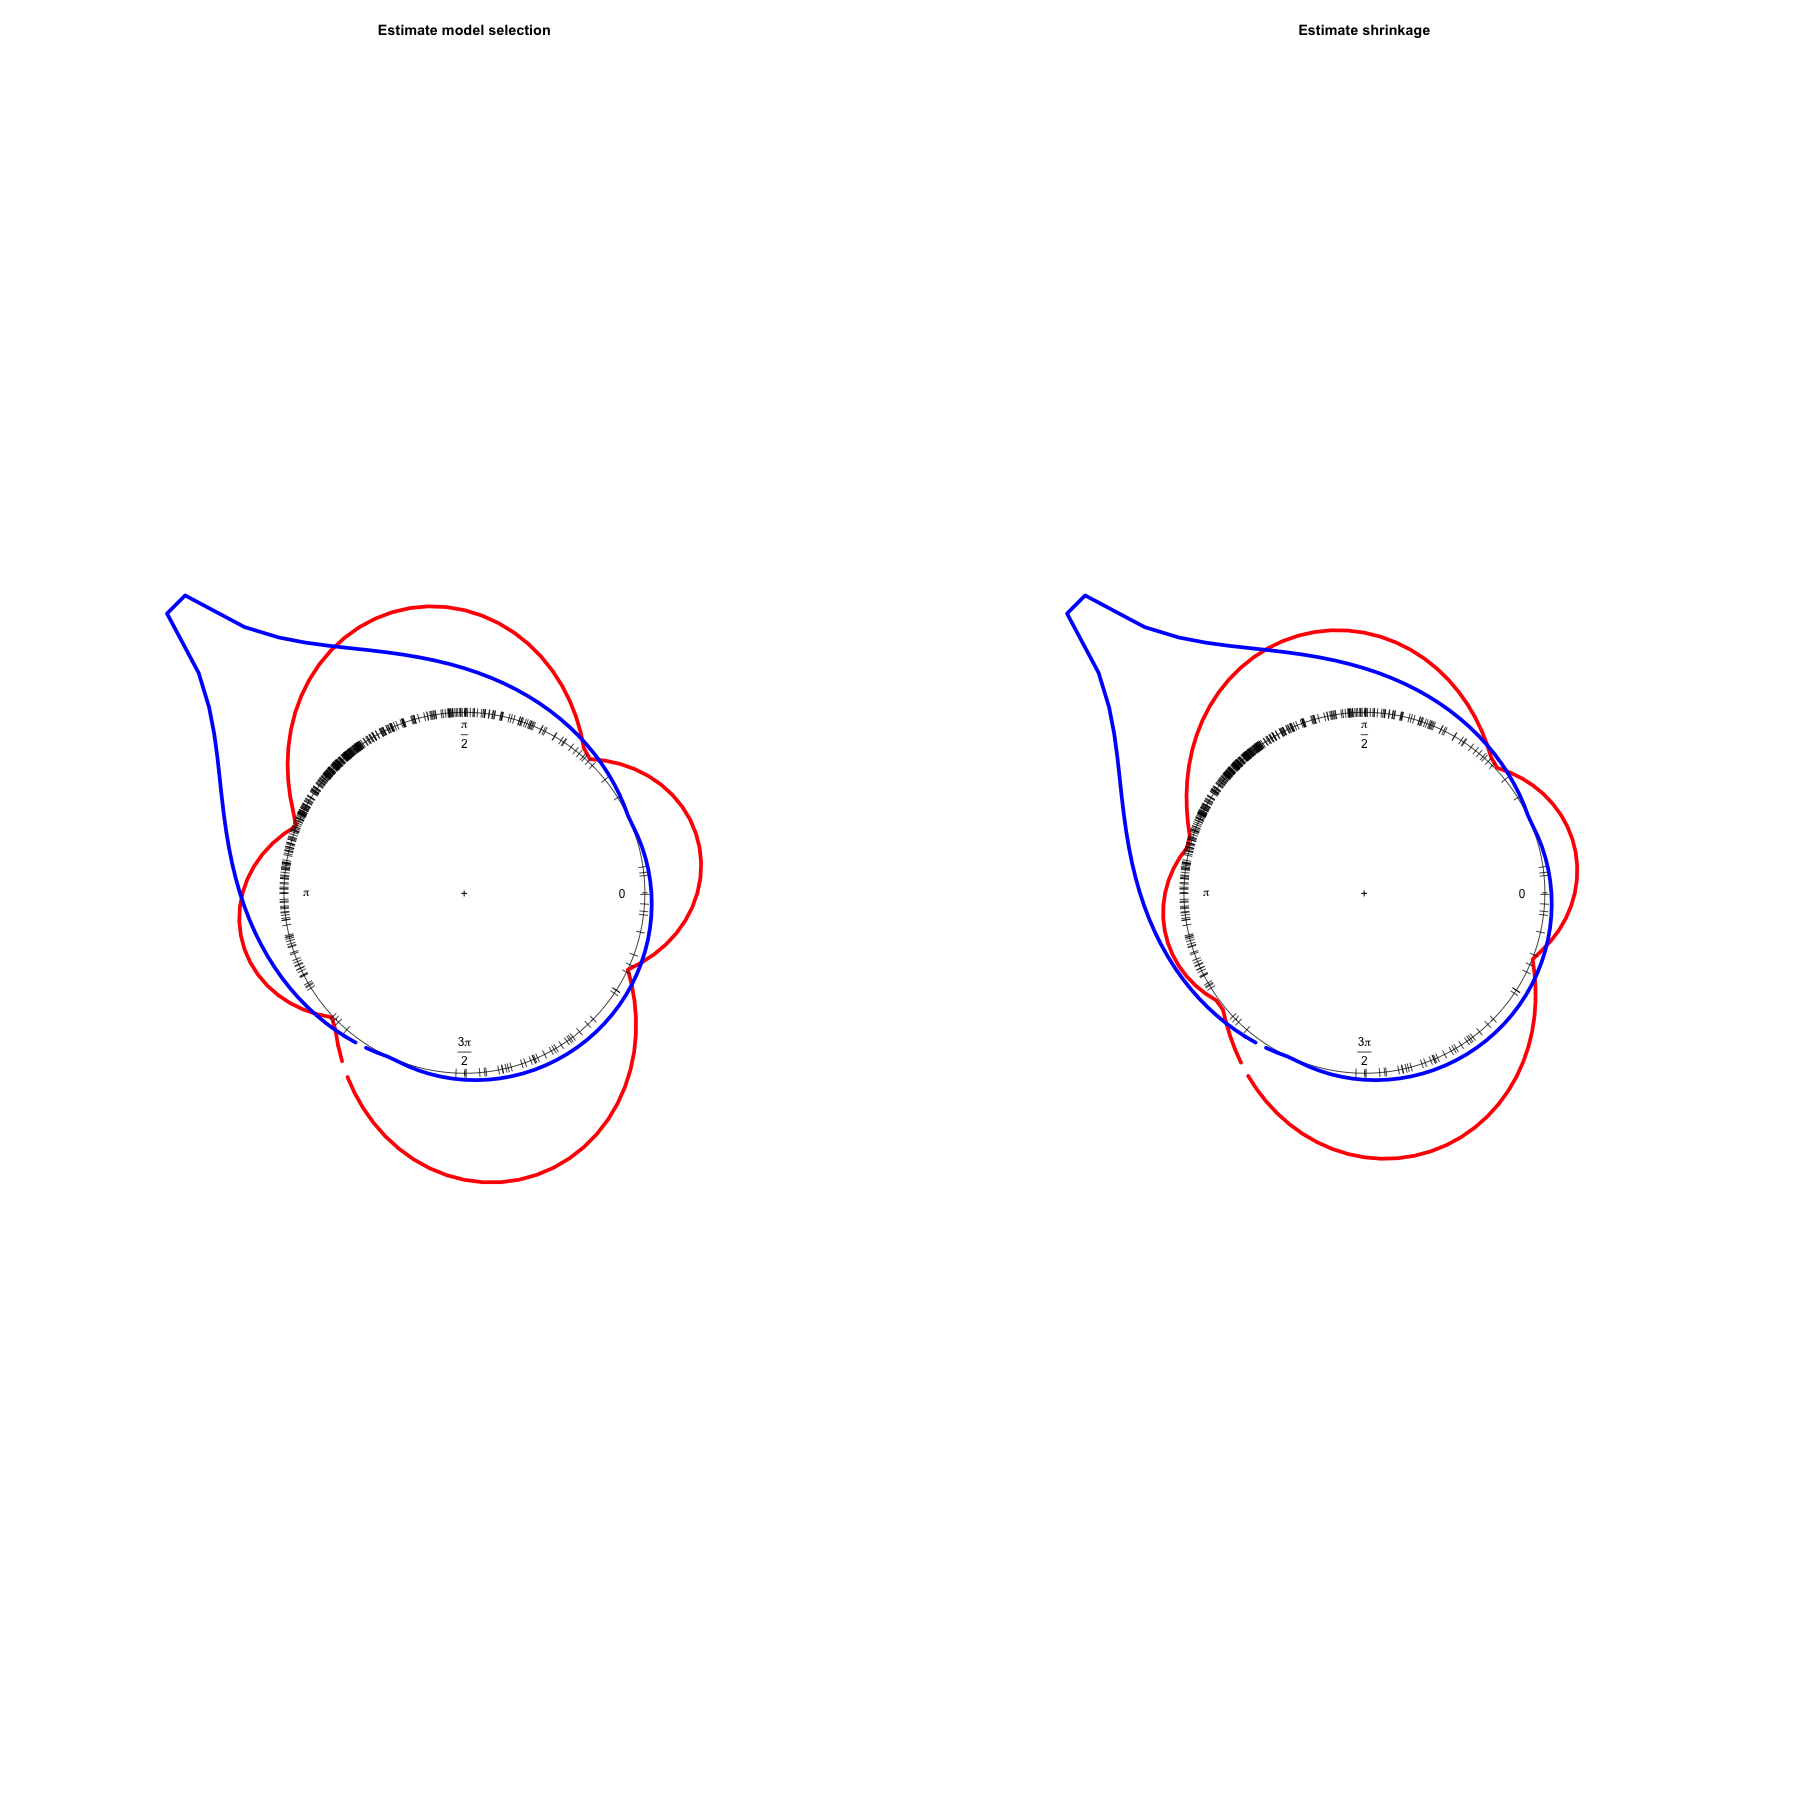
\includegraphics[width=.49\linewidth]{density/distM/50.png} \\[\abovecaptionskip]
  \end{tabular}
  \caption{Evolution of the aggregation weights }
  \label{fig:ge:adaptive:M}
\end{figure}

\medskip

Consider first the asymptotic when one lets $\eta$ tend to infinity.
Under \nref{AS_INTRO_DATA_KNOWN}, following a model selection approach (c.f. \ncite{barron1999risk} and \ncite{Massart2007} for an extensive description), a dimension parameter $\hDi$ is determined among a collection of admissible values $\nset{1,\ssY}$ by minimising the penalised contrast function $-\Vnormlp{\txdfPr}+\penSv$, that is
\begin{equation}\label{freq:ge:shape:kn:de:ms}
  \tDi:=\argmin\nolimits_{\Di\in\nset{1,\ssY}} \big\{-\Upsilon(m) + \penSv\big\}.
\end{equation}
If $\tDi$ minimises uniquely the penalised contrast function, then it is easily seen that the discrete probability measure $\rWe[]$ on the set $\nset{1,\ssY}$ given by the weights $\rWe[](\{\Di\})=\rWe$ as in \eqref{freq:ge:shape:kn:we} degenerates to a Dirac measure $\dirac[\tDi]$ on the point $\tDi$ as $\rWc\to\infty$.
Precisely, for any $\Di\in\nset{1,n}$ holds
\begin{equation}\label{freq:ge:shape:kn:de:msWe}
  \lim\nolimits_{\rWc\to\infty}\rWe=\dirac[\tDi](\{\Di\})=:\msWe
\end{equation}
Thereby, in the sequel we consider the model selected estimator
\[\txdfPr[\tDi]=\widehat{\theta}^{(\infty)} =\sum\nolimits_{\Di\in\nset{1,\ssY}}\msWe\txdfPr\]
as an aggregation with respect to the discrete measure $\msWe[]=\dirac[\tDi]$ on the set $\nset{1,\ssY}$.
We give in \nref{fig:ge:adaptive:selection} an illustration of the model selection estimator used on a Gaussian sequence space model, in the direct problem case, that is to say $\lambda(s) = 1$ for all $s$.

\begin{figure}
\centering
  \begin{tabular}{@{}c@{}}
    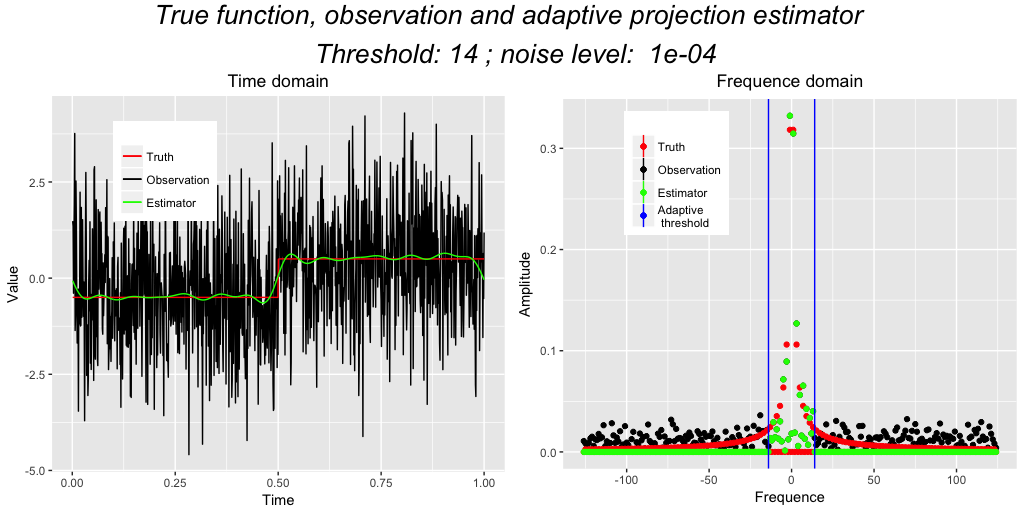
\includegraphics[width=.49\linewidth]{gauss/adaptive/model_selection.png} \\[\abovecaptionskip]
  \end{tabular}
  \begin{tabular}{@{}c@{}}
    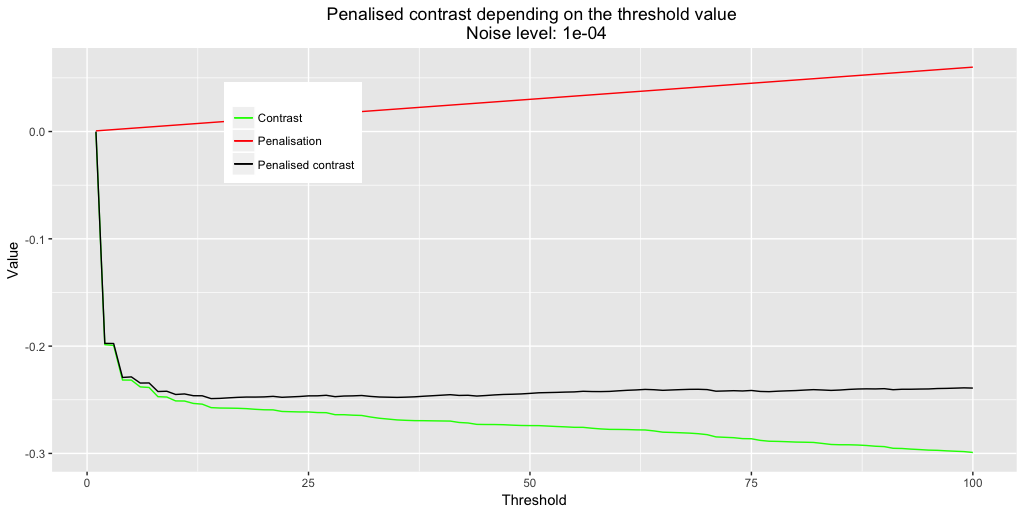
\includegraphics[width=.49\linewidth]{gauss/adaptive/penalised_contrast.png} \\[\abovecaptionskip]
  \end{tabular}
  \caption{Model selection estimator on an Gaussian sequence space model, direct problem case}
  \label{fig:ge:adaptive:selection}
\end{figure}

Under \nref{AS_INTRO_DATA_UNKNOWN} consider again a  model selection approach by
minimising now the penalised contrast function $\Upsilon(m)+\peneSv$, that is
\begin{equation}\label{freq:ge:shape:uk:de:ms}
  \hDi:=\argmin_{\Di\in\nset{1,\ssY}} \big\{-\Upsilon(m)+\peneSv\big\}.
\end{equation}
If $\hDi$ minimises uniquely the penalised contrast function, then for any $\Di\in\nset{1,n}$ holds
\begin{equation}\label{freq:ge:shape:uk:de:msWe}
  \lim_{\rWc\to\infty}\erWe=\dirac[\hDi](\{\Di\})=:\widehat{\P}_{M}^{(\infty)}.
\end{equation}
Thereby, we consider again the model selected estimator

$\txdfPr[\tDi] = \widehat{\theta}^{(\infty)} = \sum_{\Di\in\nset{1,\ssY}}\widehat{\P}_{M}^{(\infty)}(m)\hxdfPr$ as an aggregation with respect to the discrete measure $\msWe[]=\dirac[\hDi]$ on the set $\nset{1,\ssY}$.

We will consider two examples in this chapter, namely the inverse Gaussian sequence space model as well as the circular deconvolution model.
In both cases the functions $\Upsilon$, $\pen^{\Lambda}$, and $\pen^{\widehat{\Lambda}}$ take the same shape which we hence give here.
\begin{de}\label{freq:ge:shape:kn:de:pen:oo}
  Under \nref{AS_INTRO_DATA_KNOWN}, let be a universal constant $\cpen$ to be fixed depending on the considered model.
  For any $\Di$ in $\nset{1,\ssY}$, remind that $\Lambda(m) = \vert \lambda(m) \vert^{-2}$, and $\Lambda_{+}(m) = \max\{\Lambda(s), s \in \mathds{F}_{m} \}$ and define
  \begin{alignat*}{4}
  & \Upsilon(m) && := && \Vert \theta_{n, \overline{m}} \Vert_{l^{2}}^{2};  \quad && \cmiSv := \tfrac{\log^{2}(\Di\miSv \vee(\Di+2))}{\log^{2}(\Di+2)}\geq1;\\
  & \DipenSv && := && \cmiSv \Di \miSv; \quad && \penSv:= \penD.
  \end{alignat*}
  \assEnd
\end{de}
\begin{de}\label{freq:ge:shape:uk:de:pen:oo}
  Under \nref{AS_INTRO_DATA_UNKNOWN}, let be a universal constant $\cpen$ to be fixed depending on the considered model.
  Then, for any $m$ in $\N$, we define
  \begin{alignat*}{4}
  & \Upsilon(m) && := && \Vert \theta_{n, n_{\lambda}, \overline{m}}\Vert_{l^{2}}^{2}; && \quad \eiSv[(s)]:= \vert \hfedfmpI[(s)] \vert ^2\\
    & \meiSv && := && \max\{\eiSv[(l)],l\in\nset{1,\Di}\}; && \quad \cmeiSv:=\tfrac{\log^{2}(\Di\meiSv\vee(\Di+2))}{\log^{2}(\Di+2)}\geq1;\\
    &\DipeneSv && := && \cmeiSv \Di \meiSv;&& \quad \peneSv:= \peneD.
  \end{alignat*}
  \assEnd
\end{de}
Notice that, with the exception of the constant $\kappa$, our estimator is now fully determined, in both cases \nref{AS_INTRO_DATA_KNOWN} and \nref{AS_INTRO_DATA_UNKNOWN}.

\section{Strategy of proof for optimality of aggregation estimator}\label{freq:ge:strat}\label{FREQ_STRATEGY}
As we have now given a precise shape to our aggregation estimator, we propose a strategy to compute upper bounds for its convergence rate in $l^{2}$-norm.
Our method is inspired by the strategy to compute upper bounds for the contraction rate of hierarchical sieves we presented in the previous chapter.
We will hence highlight a decomposition of the risk which separates the risk obtained by taking values of the threshold which are respectively "too small", "too large", or "optimal".
Those terms should be understood with respect to the quadratic risk of the projection estimator associated with this choice of threshold.
One would then prove that the values of the threshold which are too small or too large do not receive an important weight under $\P_{M}^{(\eta)}$ or $\widehat{P}_{M}^{(\eta)}$.
Before going any further, notice that, for any $\Di$ and $m^{\bullet}$ in $\N$, the aggregation weights can be bounded in the following way:
\begin{multline*}
\tfrac{\exp[-\eta n (-\Vert \theta_{n, \overline{m}} \Vert_{l^{2}} + \pen^{\Lambda}(m))]}{\sum\nolimits_{k = 0}^{n} \exp[-\eta n (-\Vert \theta_{n, \overline{k}} \Vert_{l^{2}} + \pen^{\Lambda}(k))]} \mathds{1}_{m \leq n}\\
\leq \exp[-\eta n (\Vert \theta_{n, \overline{m}} \Vert_{l^{2}} - \Vert \theta_{n, \overline{m^{\bullet}}} \Vert_{l^{2}} + \pen^{\Lambda}(m^{\bullet}) - \pen^{\Lambda}(m))] \mathds{1}_{m \leq n}\text{; and}
\end{multline*}
\begin{multline*}
\tfrac{\exp[-\eta n (-\Vert \theta_{n, n_{\lambda}, \overline{m}} \Vert_{l^{2}} + \pen^{\Lambda}(m))]}{\sum\nolimits_{k = 0}^{n} \exp[-\eta n (-\Vert \theta_{n, n_{\lambda}, \overline{k}} \Vert_{l^{2}} + \pen^{\Lambda}(k))]} \mathds{1}_{m \leq n}\\
\leq \exp[-\eta n (\Vert \theta_{n, n_{\lambda}, \overline{m}} \Vert_{l^{2}} - \Vert \theta_{n, n_{\lambda}, \overline{m^{\bullet}}} \Vert_{l^{2}} + \pen^{\Lambda}(m^{\bullet}) - \pen^{\Lambda}(m))] \mathds{1}_{m \leq n}.
\end{multline*}

Then, the following lemma, which proof is given in \nref{pro:re:contr} allows to derive an upper bound which is easier to control.

\begin{lm}\label{re:contr}
Given $\ssY\in\Nz$ and $\xdfPr[],\dxdfPr[]\in\lp[2]$ consider the
  families of  orthogonal projections
  
  $\setB{\dxdfPr=\dProj{\Di}{}\dxdfPr[],\Di\in\nset{1,n}}$ and $\setB{\xdfPr=\dProj{\Di}{}\xdf,\Di\in\nset{1,n}}$.
  
  If $\Vnormlp{\dProj{\Di}{}^\perp\xdf}^2=\Vnormlp{\xdf_{\underline{0}}}^2\bias^2(\xdf)$ for all
  $\Di\in\nset{1,\ssY}$, then for any $l\in\nset{1,n}$ holds
 \begin{resListeN}[]
\item\label{re:contr:e1}
$\Vnormlp{\dxdfPr[k]}^2-\Vnormlp{\dxdfPr[l]}^2\leq
\tfrac{11}{2}\Vnormlp{\dxdfPr[l]-\xdfPr[l]}^2-\tfrac{1}{2}\Vnormlp{\xdf_{\underline{0}}}^2\{\bias[k]^2(\xdf)-\bias[l]^2(\xdf)\}$,
for all $k\in\nsetro{1,l}$;
\item\label{re:contr:e2}
$\Vnormlp{\dxdfPr[k]}^2-\Vnormlp{\dxdfPr[l]}^2\leq \tfrac{7}{2}\Vnormlp{\dxdfPr[k]-\xdfPr[k]}^2+\tfrac{3}{2}\Vnormlp{\xdf_{\underline{0}}}^2
\{\bias[l]^2(\xdf)-\bias[k]^2(\xdf)\}$, for all $k\in\nsetlo{l,n}$.
\end{resListeN}
\reEnd
\end{lm}

\subsection{Known operator}\label{freq:ge:strat:kn}\label{FREQ:GE:STRAT:KN}
Consider first the case \nref{AS_INTRO_DATA_KNOWN}.
We shall hence keep in mind \ref{freq:ge:shape:kn}, \ref{freq:ge:shape:kn:we}, \nref{freq:ge:shape:kn:de:pen:oo} as well as \ref{freq:ge:shape:kn:de:ms} and \ref{freq:ge:shape:kn:de:msWe}.
\textbf{Note that the detailed proofs for all results given here can be found in \nref{pro:freq:ge:strat:kn}}.

Both for the quadratic and the maximal risk, our strategy is based on the decomposition of the quadratic loss function displayed in \nref{freq:ge:strat:kn:co:agg}.
This decomposition is independent of the model and only relies on the fact that the parameter space is equipped with a nested sieve and the fact that our estimator aggregation structure takes advantage of it.
\begin{lm}\label{freq:ge:strat:kn:co:agg}
First writing the $l^{2}$-distance between $\theta^{\circ}$ and $\widehat{\theta}^{\eta}$ we obtain, for any $\mDi$ and $\pDi$ in $\llbracket 1, n \rrbracket$ such that $\mDi \leq \pDi$, and sequence $(\pen(m))_{m \in \N}$ of compensating terms,
\begin{multline}\label{freq:ge:strat:kn:co:agg:e1}
    \Vnormlp{\txdfAg-\xdf}^2\leq \tfrac{2}{7}\pen(\pDi) +2\Vnormlp{\xdf_{\underline{0}}}^2\bias[\mDi]^2(\xdf)\\\hfill
    +2\Vnormlp{\xdf_{\underline{0}}}^2\We[](\nsetro{1,\mDi})+\tfrac{2}{7}\sum\nolimits_{\Di\in\nsetlo{\pDi,\ssY}}\pen(m)\We\Ind{\{\Vnormlp{\txdfPr-\xdf_{\overline{m}}}^2<\pen(\Di)/7\}}\\
+2\sum_{\Di\in\nset{\pDi,\ssY}}\vectp{\Vnormlp{\txdfPr-\xdf_{\overline{m}}}^2-\pen(\Di)/7}  
+\tfrac{2}{7}\sum_{\Di\in\nsetlo{\pDi,\ssY}}\pen(\Di)\Ind{\{\Vnormlp{\txdfPr-\xdf_{\overline{m}}}^2\geq \pen(m)/7\}}.
\end{multline}
\reEnd
\end{lm}
The proof strategy will be articulated around the search for sequences $\pDi$, $\mDi$ and $\pen(m)$ such that each term is properly controlled.
In practice, the terms $\tfrac{2}{7}\pen(\pDi)$ and $2\Vnormlp{\xdf_{\underline{0}}}^2\bias[\mDi]^2(\xdf)$ will be the leading terms in the sum.

\subsubsection{Quadratic risk bounds}\label{freq:ge:strat:kn:qu}
We propose a strategy which allows to prove that the sequence defined hereafter is an upper bound for the quadratic risk of the aggregation estimator we just defined.
\begin{de}\label{freq:ge:strat:kn:qu:de:rate}
Remind that we defined for any $\theta$ in $\Theta$ and $\Di$ in $\N$ the following term $\b_{m}^{2}(\theta) = \Vert \theta_{\underline{m}} \Vert_{l^{2}}^{2}\Vert \theta_{\underline{0}} \Vert_{l^{2}}^{-2} \leq 1$.
We then define a family of sequences $(\daRa{\Di}{(\xdf)})_{\Di \in \N} := (\daRa{\Di}{(\xdf,\Lambda)})_{\Di \in \N} = ([\b_{m}^{2}(\theta^{\circ}) \vee \penSv/\cpen])_{\Di \in \N}$ and hence it holds for all $\Di$ in $\nset{1,\ssY}$
    \begin{equation}\label{freq:ge:strat:kn:qu:de:rate:e1}
      [\Vnormlp{\xdf_{\underline{0}}}^2+\cpen]\daRa{\Di}{(\xdf)}\geq\Vnormlp{\xdf_{\underline{0}}}^2\bias^2(\xdf)\vee\penSv.
      \end{equation}
We intend to prove that the specific choice
\begin{multline*}
\aDi{\ssY}(\xdf):=\argmin\Nset[\Di\in\Nz]{\daRa{\Di}{(\xdf)}}\in\nset{1,\ssY}; \\
\naRa{(\xdf)}:=\naRa{(\xdf,\Lambda)}:=\min\Nset[\Di\in\Nz]{\daRa{\Di}{(\xdf)}}
\end{multline*}
with $\daRa{\aDi{\ssY}}{(\xdf,\Lambda)}=\naRa{(\xdf,\Lambda)}$ defines an upper bound for the convergence rate of the aggregation estimators.
\assEnd
\end{de}
Note that the proofs for the results displayed here can be found in \nref{pro:freq:ge:strat:kn:qu}
\begin{rmk}\label{freq:ge:strat:kn:qu:rmk:rate} The following statements can be
shown using the same   arguments as in \nref{oo:rem:ora}
by exploiting that the sequence $\bias^2(\xdf)$ is non-increasing with limit zero and $\bias[0]^2(\xdf)\leq1$. 
By construction  for all $\ssY\in\Nz$ it hold 
$\naRa{(\xdf)}\geq \ssY^{-1}$ and $\naRa{(\xdf)}=\mathfrak{o}_{n}(1)$.
Moreover, for all $\ssY\in\Nz$ we have $\aDi{\ssY}(\xdf)\in\nset{1,\ssY}$,
$\aDi{\ssY}(\xdf)=\argmin\Nset[{\Di\in\nset{1,\ssY}}]{\daRa{\Di}{(\xdf)}}$ and 
$\naRa{(\xdf)}=\min\Nset[{\Di\in\nset{1,\ssY}}]{\daRa{\Di}{(\xdf)}}$. 
Thereby, in case \ref{oo:xdf:p} we conclude that $\aDi{\ssY}(\xdf)=K$ and
the rate $\naRa{(\xdf)}$ is parametric, that is
$\naRa{(\xdf)}=\DipenSv[K]\ssY^{-1}\approx\ssY^{-1}$, and hence
equals the oracle rate $\oRa{\xdf}$, i.e. $\oRa{\xdf}\approx\naRa{(\xdf)}$. On the other
hand side, in case \ref{oo:xdf:np}  the rate
$\naRa{(\xdf)}$ is nonparametric, that is,
$\ssY\naRa{(\xdf)}\to\infty$ and $\aDi{\ssY}(\xdf)\to\infty$  as
$\ssY\to\infty$. Moreover, by construction holds $\naRa{(\xdf)}\geq\oRa{\xdf}$.
 \remEnd
\end{rmk}

\begin{te}
 Let us first briefly illustrate the last definitions by stating the
 order of $\aDi{\ssY}(\xdf)$ and $\naRa{(\xdf)}$ in the cases considered
 in \nref{il:oo}
\end{te}
% ....................................................................
% <<Il upper bound oo>>
% ....................................................................
\begin{il}\label{freq:ge:strat:kn:qu:il:rate}Let us illustrate  \nref{freq:ge:strat:kn:qu:de:rate}
  considering as in \nref{il:oo} usual behaviour \ref{il:oo:oo},
  \ref{il:oo:so} and \ref{il:oo:os} for the sequences
  $\Nsuite[\Di]{\bias[\Di](\xdf)}$ and $\Nsuite[\Di]{\iSv[\Di]}$:
  \begin{Liste}[]
  \item[\mylabel{freq:ge:strat:kn:qu:il:rate:np:oo}{\dg\bfseries{[o-o]}}] Since
    $\bias^2(\xdf)\approx\Di^{-2p}$ and $\DipenSv\approx\Di^{2a+1}$ follows
    $\daRa{\aDi{\ssY}}{(\xdf,\Lambda)}\approx(\aDi{\ssY})^{-2p}\approx\DipenSv[\aDi{\ssY}]\ssY^{-1}\approx(\aDi{\ssY})^{2a+1}\ssY^{-1}$
    which implies $\aDi{\ssY}\approx\ssY^{1/(2p+2a+1)}$,
    $\cmiSv[\aDi{\ssY}]\aDi{\ssY}\approx\ssY^{1/(2p+2a+1)}$,
    $\naRa{(\xdf)}\approx\ssY^{-2p/(2p+2a+1)}$ and
    $ \vert \log\naRa{(\xdf)} \vert \approx(\log\ssY)$.
  \item[\mylabel{freq:ge:strat:kn:qu:il:rate:np:os}{\dg\bfseries{[o-s]}}] Since
    $\bias^2(\xdf)\approx\Di^{-2p}$ and
    $\DipenSv\approx\Di^{1+4a}\exp(\Di^{2a})$ follows
    $\daRa{\aDi{\ssY}}{(\xdf,\Lambda)}\approx(\aDi{\ssY})^{-2p}\approx\DipenSv[\aDi{\ssY}]\ssY^{-1}\approx(\aDi{\ssY})^{1+4a}\exp((\aDi{\ssY})^{2a})$
    which implies $\aDi{\ssY}\approx(\log\ssY)^{1/(2a)}$,
    $\cmiSv[\aDi{\ssY}]\aDi{\ssY}\approx(\log\ssY)^{2+1/(2a)}$,
    $\naRa{(\xdf)}\approx(\log\ssY)^{-p/a}$ and
    $ \vert \log\naRa{(\xdf)} \vert \approx(\log\log\ssY)$.
  \item[\mylabel{freq:ge:strat:kn:qu:il:rate:np:so}{\dg\bfseries{[s-o]}}] Since
    $\bias^2(\xdf)\approx\exp(-\Di^{2p})$ and $\DipenSv\approx\Di^{2a+1}$
    follows
    $\daRa{\aDi{\ssY}}{(\xdf,\Lambda)}\approx\exp(-(\aDi{\ssY})^{2p})\approx\DipenSv[\aDi{\ssY}]\ssY^{-1}\approx
    (\aDi{\ssY})^{2a+1}\ssY^{-1}$ which implies
    $\aDi{\ssY}\approx(\log\ssY)^{1/(2p)}$,
    $\cmiSv[\aDi{\ssY}]\aDi{\ssY}\approx(\log\ssY)^{1/(2p)}$,
    $\naRa{(\xdf)}\approx(\log\ssY)^{(2a+1)/(2p)}\ssY^{-1}$ and
    $ \vert \log\naRa{(\xdf)} \vert \approx(\log\ssY)$.
  \end{Liste}
  We note that  in the three cases \ref{freq:ge:strat:kn:qu:il:rate:np:oo},
  \ref{freq:ge:strat:kn:qu:il:rate:np:os} and \ref{freq:ge:strat:kn:qu:il:rate:np:so} the rate
  $\naRa{(\xdf)}$ coincide with the
  oracle rate $\oRa{\xdf}$ derived in \nref{il:oo} \ref{il:oo:oo},
  \ref{il:oo:os} and \ref{il:oo:so}, respectively.\ilEnd 
\end{il}
% ....................................................................
% Define *Di
% ....................................................................
\begin{te}
  Under \nref{freq:ge:shape:kn:de:pen:oo} for arbitrary $\pdDi,\mdDi \in \nset{1,\ssY}$ let us define
  \begin{multline}\label{freq:ge:strat:kn:qu:de:mDipDi}
    \mDi:=\min\set{\Di\in\nset{1,\mdDi}: \Vnormlp{\xdf_{\underline{0}}}^2\bias^2(\xdf) \leq [\Vnormlp{\xdf_{\underline{0}}}^2+4\cpen]\daRa{\mdDi}{(\xdf)}}\quad\text{and}\\
    \pDi:=\max\set{\Di\in\nset{\pdDi,\ssY} : \penSv \leq 2[3\Vnormlp{\xdf_{\underline{0}}}^2 + 2\cpen] \daRa{\pdDi}{(\xdf)}}
  \end{multline}
  where the defining set obviously contains $\mdDi$ and $\pdDi$, respectively, and hence, it is not empty.
\end{te}
\begin{te}
Considering the third and fourth terms on the right hand side of \eqref{freq:ge:strat:kn:co:agg:e1}, we will use the following lemma to control them.
\end{te}
% ....................................................................
% <<Re Sum Random weights>>
% ....................................................................
\begin{lm}\label{freq:ge:strat:kn:qu:re:SrWe:ag}
Consider the data-driven aggregation weights $\rWe[]$
  as in \eqref{freq:ge:shape:kn:we}.  Under \nref{freq:ge:shape:kn:de:pen:oo} with
  $\cpen\geq8\log(3e)$ for any
  $\mdDi,\pdDi\in\nset{1,\ssY}$ and associated $\pDi,\mDi\in\nset{1,\ssY}$
  as in \eqref{freq:ge:strat:kn:qu:de:mDipDi} hold
  \begin{resListeN}
  \item\label{freq:ge:strat:kn:qu:re:SrWe:ag:i}
    $\rWe[](\nsetro{1,\mDi})
    \Ind{\setB{\Vnormlp{\txdfPr[\mdDi]-\xdfPr[\mdDi]}^2<\cpen\daRa{\mdDi}{(\xdf)}/7}}\leq
    \tfrac{1}{\rWc\cpen}\Ind{\{\mDi>1\}}
    \exp\big(-\tfrac{3\rWc\cpen}{14} \ssY\daRa{\mdDi}{(\xdf)}\big)$;
  \item\label{freq:ge:strat:kn:qu:re:SrWe:ag:ii}
    $\sum_{\Di\in\nsetlo{\pDi,\ssY}}\penSv\rWe
    \Ind{\{\Vnormlp{\txdfPr[\Di]-\xdfPr[\Di]}^2<\penSv/7\}}
    \leq \ssY^{-1}\{\tfrac{16}{\cpen\rWc^{2}}+ \tfrac{8}{\rWc}\}$.
  \end{resListeN}\reEnd
\end{lm}
% ....................................................................
% <<Te Sum MS Random weights>>
% ....................................................................
\begin{te}
  We combine the upper bound in \nref{freq:ge:strat:kn:co:agg} and the bounds given in \nref{freq:ge:strat:kn:qu:re:SrWe:ag}.
  Clearly, due to \nref{freq:ge:strat:kn:qu:re:SrWe:ag} we have
  \begin{displaymath}
    \E\rWe[](\nsetro{1,\mDi})\leq\Ind{\{\mDi>1\}} \{\tfrac{1}{\rWc\cpen}\exp\big(-\tfrac{3\rWc\cpen}{14}n\daRa{\mdDi}{(\xdf)}\big) + \P\big(\Vnormlp{\txdfPr[\mdDi]-\xdfPr[\mdDi]}^2 \geq \tfrac{\cpen}{7}\daRa{\mdDi}{(\xdf)}\big)\}
  \end{displaymath}
  and, hence from \eqref{freq:ge:strat:kn:co:agg} follows immediately
  \begin{multline}\label{freq:ge:strat:kn:qu:e1}
    \E\Vnormlp{\txdfAg-\xdf}^2\leq \ssY^{-1} \{\tfrac{32}{7\cpen\rWc^{2}} + \tfrac{16}{7\rWc}\} + \tfrac{2}{\rWc\cpen}\Vnormlp{\xdf_{\underline{0}}}^2\Ind{\{\mDi>1\}} \exp\big(-\tfrac{3\rWc\cpen}{14}n\daRa{\mdDi}{(\xdf)}\big)\\
    \hfill + 2\Vnormlp{\xdf_{\underline{0}}}^2\Ind{\{\mDi>1\}} \P\big(\Vnormlp{\txdfPr[\mdDi] - \xdfPr[\mdDi]}^2 \geq \tfrac{\cpen}{7} \daRa{\mdDi}{(\xdf)} \big) + \tfrac{2}{7} \penSv[\pDi]  + 2 \Vnormlp{\xdf_{\underline{0}}}^2 \bias[\mDi]^2(\xdf) \\
     +2\sum_{\Di\in\nset{\pdDi,n}}\E\vectp{\Vnormlp{\txdfPr-\xdfPr}^2-\tfrac{1}{7}\penSv}\\
    +\tfrac{2}{7}\sum_{\Di\in\nset{\pdDi,\ssY}}\penSv
    \P\big(\Vnormlp{\txdfPr-\xdfPr}^2\geq\tfrac{1}{7}\penSv\big)
  \end{multline}
\end{te}
% ....................................................................
% Outline Oracle optimality
% ....................................................................
\begin{te}
 The next result can be directly deduced from \nref{freq:ge:strat:kn:qu:re:SrWe:ag} by letting $\rWc\to\infty$.
 However, we think the direct proof given in \nref{pro:freq:ge:strat:kn} provides an interesting illustration of the values $\pDi,\mDi\in\nset{1,\ssY}$ as defined in \eqref{freq:ge:strat:kn:qu:de:mDipDi}.
\end{te}
% ....................................................................
% <<Upper bound random weights>>
% ....................................................................
\begin{lm}\label{freq:ge:strat:kn:qu:re:SrWe:ms}
Consider the data-driven model selection weights $\msWe[]$ as in \eqref{freq:ge:shape:kn:de:msWe}.
Under definition \nref{freq:ge:shape:kn:de:pen:oo} for any $\mdDi,\pdDi\in\nset{1,\ssY}$ and associated $\pDi,\mDi\in\nset{1,n}$ as in \eqref{freq:ge:strat:kn:qu:de:mDipDi} hold
\begin{resListeN}[]
  \item\label{freq:ge:strat:kn:qu:re:SrWe:ms:i}
    $\msWe[](\nsetro{1,\mDi})\Ind{\{\Vnormlp{\theta_{n, \overline{\mdDi}} - \xdfPr[\mdDi]}^2
      <\cpen\daRa{\mdDi}{(\xdf)}/7\}}=0$;
  \item\label{freq:ge:strat:kn:qu:re:SrWe:ms:ii}
    $\sum_{\Di\in\nsetlo{\pDi,\ssY}}\penSv\msWe\Ind{\{\Vnormlp{\txdfPr-\xdfPr}^2<\penSv/7\}}=0$.
  \end{resListeN}
  \reEnd
\end{lm}
% ....................................................................
% <<Te Sum MS Random weights>>
% ....................................................................
\begin{te}
We combine again the upper bound in \nref{freq:ge:strat:kn:co:agg} and the bounds given in \nref{freq:ge:strat:kn:qu:re:SrWe:ms}.
Clearly, due to \nref{freq:ge:strat:kn:qu:re:SrWe:ms} we have
$\E\msWe[](\nsetro{1,\mDi})=\P\big(\Vnormlp{\txdfPr[\mdDi]-\xdfPr[\mdDi]}^2\geq\cpen\daRa{\mdDi}{(\xdf)}/7\big)$
and, hence from \eqref{freq:ge:strat:kn:co:agg} follows immediately
  \begin{multline}\label{freq:ge:strat:kn:qu:e2}
\E\Vnormlp{\txdfPr[\hDi]-\xdf}^2\leq 2\sum\nolimits_{\Di\in\nset{\pdDi,\ssY}}\E\vectp{\Vnormlp{\txdfPr-\xdfPr}^2-\tfrac{1}{7}\penSv}\\
\hfill \tfrac{2}{7}\penSv[\pDi] + 2\Vnormlp{\xdf_{\underline{0}}}^2\bias[\mDi]^2(\xdf) + 2\Vnormlp{\xdf_{\underline{0}}}^2\Ind{\{\mDi>1\}}\P\big(\Vnormlp{\txdfPr[\mdDi]-\xdfPr[\mdDi]}^2\geq\tfrac{\cpen}{7}\daRa{\mdDi}{(\xdf)}\big)\\
+\tfrac{2}{7}\sum_{\Di\in\nset{\pdDi,\ssY}}\penSv\P\big(\Vnormlp{\txdfPr-\xdfPr}^2\geq\tfrac{1}{7}\penSv\big)
\end{multline}
The deviations of the last three terms in the last display \eqref{freq:ge:strat:kn:qu:e2} and also in
\eqref{freq:ge:strat:kn:qu:e1} we bound by exploiting usual concentration inequalities which depend on the model considered.
We hence formulate this property as the assumption to be verified in order to use this strategy.
\end{te}

\begin{as}\label{freq:ge:strat:kn:qu:as}
Remind that we defined $\oiSv=\tfrac{1}{\Di}\sum_{s\in\nset{1,\Di}}\iSv[s]$,

$\miSv= \max\{\iSv[s],s\in\nset{1,\Di}\}$, $\cmSv\geq1$ and $\DipenSv=\cmSv\Di \miSv$.
Assume that there are numerical constants $(\cst{i})_{1 \in \llbracket 1, 11 \rrbracket}$, such that for all $\ssY\in\Nz$ and $\Di\in\nset{1,\ssY}$ holds
  \begin{resListeN}[]
  \item\label{freq:ge:strat:kn:qu:as:i}
    $\E \vectp{\Vnormlp{\txdfPr-\xdfPr}^2 - 12\tfrac{\DipenSv}{\ssY}}  \leq 
    \cst{1} \bigg[\tfrac{\cst{2} \, \miSv}{\ssY}\exp\big(-\cmSv\Di\cst{3} \big)+\tfrac{\cst{4}\Di\miSv}{n^2}\exp\big(- \cst{5} \sqrt{n\cmSv}\big) \bigg]$
  \item\label{freq:ge:strat:kn:qu:as:ii}
    $\P\big(\Vnormlp{\txdfPr-\xdfPr}^2 \geq 12\DipenSv\ssY^{-1}\big)\leq 
    \cst{6} \bigg[\exp\big(-\cst{7} \cmSv\Di\big)
    +\exp\big(-\cst{8} \sqrt{\ssY\cmSv}\big)\bigg]$
  \item\label{freq:ge:strat:kn:qu:as:iii}
    $\P\big(\Vnormlp{\txdfPr-\xdfPr}^2 \geq 12\daRa{\Di}{(\xdf,\Lambda)}\big)\leq 
    \cst{9} \bigg[\exp\big(\tfrac{-\cst{10} \ssY\daRa{\Di}{(\xdf,\Lambda)}}{\miSv}\big)
    +\exp\big(\tfrac{-\cst{11} \ssY\sqrt{\daRa{\Di}{(\xdf,\Lambda)}}}{\sqrt{\Di\miSv}}\big)\bigg]$
  \end{resListeN}
\end{as}

\begin{te} Consider now the partially data-driven aggregation of the
  orthogonal series estimators using either  aggregation weights $\rWe[]$
  as in \eqref{freq:ge:shape:kn:we} or model selection weights $\msWe[]$ as in \eqref{freq:ge:shape:kn:de:msWe}
  combining \nref{freq:ge:strat:kn:qu:as} and the upper bound given
  in \eqref{freq:ge:strat:kn:qu:e1}  or \eqref{freq:ge:strat:kn:qu:e2} we obtain the next result, which proof is immediate and we omit it.
\end{te}

\begin{lm}\label{ak:re:nd:rest}
Assume that \nref{freq:ge:strat:kn:qu:as} holds true and use the penalty described in \nref{freq:ge:shape:kn:de:pen:oo} with $\kappa \geq 84$ so that $\penSv/7 \geq 12 n^{-1} \Delta_{\Lambda}(m)$for any $m$ in $\llbracket 1, n \rrbracket$.
Then, for all $\ssY\in\Nz$ and $\Di\in\nset{1,\ssY}$ hold
  \begin{resListeN}[]
  \item\label{ak:re:nd:rest1} let $\Di_{\cst{3}}:=\floor{  3(2/\cst{3})^2}$ and $\ssY_{\cst{5}}:={15(\cst{5})^{-4}}$ then\\ 
    $\sum_{\Di=1}^{\ssY}\E
    \vectp{\Vnormlp{\txdfPr-\xdfPr}^2-\penSv/7}
    \leq \cst{1}\ssY^{-1}\big[\tfrac{2 \cst{2}}{\cst{3}}\miSv[\Di_{\cst{3}}] + \cst{4} \ssY_{\cst{5}} \miSv[\ssY_{\cst{5}}]\big]$
  \item\label{ak:re:nd:rest2} let
    $\Di_{\cst{7}}:=\floor{3(2 / \cst{7})^2}$ and
    $\ssY_{\cst{8}}:=15(3/\cst{8})^4$ then
    \begin{multline*}
    \sum_{\Di=1}^{\ssY}\penSv/7\P\big(\Vnormlp{\txdfPr-\xdfPr}^2\geq\penSv/7\big)\\
    \leq\cst{6} n^{-1} \big[\miSv[\Di_{\cst{7}}]^2\Di_{\cst{7}}^2+\miSv[\ssY_{\cst{8}}]^2 \ssY_{\cst{8}}^{2}\big]
    \end{multline*}
  \item\label{ak:re:nd:rest3} 
  $\P\big(\Vnormlp{\theta_{n, \overline{m^{\dagger}_{-}}}-\theta^{\circ}_{\overline{m^{\dagger}_{n}}}}^2 \geq 12\daRaS{\mdDi}{\xdf,\Lambda}\big)\leq 
    \cst{9} \big[\exp\big(\tfrac{-\cst{10}\ssY\daRaS{\mdDi}{\xdf,\Lambda}}{\Lambda_{+}(\mdDi)}\big)+(\cst{8})^{-2}\ssY^{-1}\big]$
  \end{resListeN}
  \reEnd
\end{lm}


Injecting \nref{ak:re:nd:rest} in either \nref{freq:ge:strat:kn:qu:e1} or \nref{freq:ge:strat:kn:qu:e2} we directly obtain the following result.

\begin{lm}\label{freq:ge:strat:kn:qu:ub}
Assume that \nref{freq:ge:strat:kn:qu:as} holds true.
Consider the penalty sequence $\penSv$ as in \nref{freq:ge:shape:kn:de:pen:oo} with numerical constant $\cpen \geq 84$.
Let $\widehat{\theta}^{(\eta)}$ be an aggregation estimator using either the aggregation weights \nref{freq:ge:shape:kn:we} or the model selection weights \nref{freq:ge:shape:kn:de:msWe}.
Let $\ssY_{\cst{5}}$, $n_{\cst{8}}$, $m_{\cst{3}}$, and $m_{\cst{7}}$ be as in \nref{{ak:re:nd:rest}}.
Then, there is a finite numerical constant $\cst{}$ such that for any $\mdDi$, $\pdDi$ and associated $\mDi$ and $\pDi$ as in \nref{freq:ge:strat:kn:qu:de:mDipDi} holds
	\begin{multline}\label{freq:ge:strat:kn:qu:ub:e1}
\E\Vnormlp{\widehat{\theta}^{(\eta)}-\xdf}^2\leq \tfrac{2}{7}\penSv[\pDi] + 2\Vnormlp{\xdf_{\underline{0}}}^2\bias[\mDi]^2(\xdf) + \cst{}\Vnormlp{\xdf_{\underline{0}}}^2\Ind{\{\mDi>1\}} \big[\exp\big(-\cst{10}\delta_{\Lambda}(\mdDi) \mdDi\big)\big]\\
 + \cst{}\big[\Vnormlp{\xdf_{\underline{0}}}^2\Ind{\{\mDi>1\}} + \miSv[\Di_{\cst{7}}]^2\Di_{\cst{7}}^2+\miSv[\ssY_{o}]^2\big]\ssY^{-1}.
\end{multline} 
\reEnd
\end{lm}
% ....................................................................
% <<Re upper bound ag>>
% ....................................................................
%\begin{lm}\label{freq:ge:strat:kn:qu:ub}
%Under \nref{freq:ge:strat:kn:qu:as}, consider the penalty sequence $\penSv:=\penD$, $\Di\in\nset{1,n}$, as in \nref{freq:ge:shape:kn:de:pen:oo}.
%Let $\widehat{\theta}^{(\eta)}=\sum_{\Di=1}^{\ssY}\We\txdfPr$ be an aggregation of the orthogonal series estimators, using either aggregation weights $\rWe[]$ as in \eqref{freq:ge:shape:kn:we}, or model selection weights $\msWe[]$ as in \eqref{freq:ge:shape:kn:de:msWe}.
%  
%There is a finite numerical constant $\cst{}>0$ such that for any $\mdDi,\pdDi\in\nset{1,n}$ and associated $\pDi,\mDi\in\nset{1,n}$ as defined in \eqref{freq:ge:strat:kn:qu:de:mDipDi} hold
%\begin{equation}\label{freq:ge:strat:kn:qu:ub:e1}
%\E\Vnormlp{\txdfPr[\hDi]-\xdf}^2\leq \cst{} \daRa{\dDi}{(\xdf)} + \tfrac{2}{7}\penSv[\pDi] + 2\Vnormlp{\xdf_{\underline{0}}}^2\bias[\mDi]^2(\xdf)
%\end{equation}
%\reEnd
%\end{lm}
% ....................................................................
% <<Te upper bound ag p np>>
% ....................................................................
\begin{te} The last bound allows us to derive an upper bound of the
  risk for  data-driven aggregated estimator  in the two cases
  \ref{oo:xdf:p} and \ref{oo:xdf:np} introduced in \nref{bm:ak}.
\end{te}
% ....................................................................
% <<Re upper bound ag p np>>
% ....................................................................
\begin{thm}\label{freq:ge:strat:kn:qu:pnp}
Under \nref{freq:ge:strat:kn:qu:as}, consider the penalty sequence $\penSv:=\penD$, $\Di\in\nset{1,n}$, as in \nref{freq:ge:shape:kn:de:pen:oo} with numerical constant $\cpen \geq 84$.
Let $\txdfAg[{\erWe[]}]=\sum_{\Di=1}^{\ssY}\We\txdfPr$ be an aggregation of the orthogonal series estimators, using either aggregation weights $\rWe[]$ as in \eqref{freq:ge:shape:kn:we}, or model selection weights $\msWe[]$ as in \eqref{freq:ge:shape:kn:de:msWe}.
\begin{Liste}[]
\item[\mylabel{ak:ag:ub:pnp:p}{\dgrau\bfseries{(p)}}]Assume there is $K\in\Nz$
  with   $1\geq \bias[{[K-1] }](\xdf)>0$ and $\bias[\Di](\xdf)=0$. For
  $K>0$ let
  $ c_{\xdf}:=\tfrac{\Vnormlp{\xdf_{\underline{0}}}^2+4\cpen}{\Vnormlp{\xdf_{\underline{0}}}^2\bias[{[K-1]}]^2(\xdf)}>1$ and
  $\ssY_{\xdf}:=\gauss{c_{\xdf}\DipenSv[K]}\in\Nz$. If
  $\ssY\in\nset{1,\ssY_{\xdf}}$ then set $\sDi{\ssY}:=\Di_{\cst{3}}\log(\ssY)$, and otherwise if
  $\ssY>\ssY_{\xdf}$ then set
  $\sDi{\ssY}:=\max\{\Di\in\nset{K,\ssY}:\ssY>c_{\xdf}\DipenSv\}$
  where the defining set contains $K$ and thus is not empty.
There is a finite constant $\cst{\xdf,\Lambda}$
given in \eqref{ak:ag:ub:pnp:p7} depending only on $\xdf$ and $\Lambda$ such that for all $n\in\Nz$ holds
\begin{equation}\label{ak:ag:ub:pnp:e1}
  \nRi{\txdfAg[{\erWe[]}]}{\xdf,\Lambda}
  % \E\Vnormlp{\txdfAg[{\erWe[]}]-\xdf}^2
  \leq
  \cst{}\Vnormlp{\xdf_{\underline{0}}}^2\big[
  \ssY^{-1}\vee\exp\big(-\cst{10}\cmiSv[\sDi{\ssY}]\sDi{\ssY}\big)\big]
  + \cst{\xdf,\Lambda}\ssY^{-1}.
\end{equation}
\item[\mylabel{ak:ag:ub:pnp:np}{\dgrau\bfseries{(np)}}] Assume that
  $\bias(\xdf)>0$ for all  $\Di\in\Nz$.
There is a finite finite constant $\cst{\xdf,\Lambda}$ given in
\eqref{ak:ag:ub:pnp:p8} depending only $\xdf$ and $\Lambda$ such that for all
$\ssY\in\Nz$  holds 
 \begin{equation}\label{ak:ag:ub:pnp:e2}
   \nRi{\txdfAg[{\erWe[]}]}{\xdf,\Lambda}
   % \E\Vnormlp{\txdfAg[{\erWe[]}]-\xdf}^2
    \leq 
   \cst{}(\Vnormlp{\xdf_{\underline{0}}}^2\vee1)\min_{\Di\in\nset{1,\ssY}}\big[\dRa{\Di}{\xdf,\Lambda}\vee\exp\big(-\cst{10}\cmiSv\Di\big)\big]\\
   +\cst{\xdf,\Lambda}\ssY^{-1}.
\end{equation}
\end{Liste}  
\end{thm}

Hence, using \nref{freq:ge:strat:kn:qu:pnp} gives us the following result.
% ....................................................................
% <<Re upper bound ag p np>>
% ....................................................................
\begin{cor}\label{ge:ak:ag:ub2:pnp}
  Let the assumptions of \nref{freq:ge:strat:kn:qu:pnp} be satisfied.
  \begin{Liste}[]
  \item[\mylabel{ge:ak:ag:ub2:pnp:p}{\dgrau\bfseries{(p)}}]
    If in addition
    \begin{inparaenum}\item[\mylabel{ge:ak:ag:ub2:pnp:pc}{{\dgrau\bfseries(A1)}}]
      there is $\ssY_{\xdf,\Lambda}\in\Nz$ such that
      $\cmiSv[\sDi{\ssY}]\sDi{\ssY}\geq (\cst{10})^{-1}(\log\ssY)$ for all
      $\ssY\geq \ssY_{\xdf,\Lambda}$
    \end{inparaenum}
    holds true, then there is a constant $\cst{\xdf,\Lambda}$ depending
    only on $\xdf$ and $\Lambda$ such that for all $n\in\Nz$ holds
    $\nRi{\txdfAg[{\erWe[]}]}{\xdf,\Lambda} \leq
    \cst{\xdf,\Lambda}\ssY^{-1}$.
  \item[\mylabel{ge:ak:ag:ub2:pnp:np}{\dgrau\bfseries{(np)}}]
    If in addition
    \begin{inparaenum}\item[\mylabel{ge:ak:ag:ub2:pnp:npc}{{\dgrau\bfseries(A2)}}]
      there is  $\ssY_{\xdf,\Lambda}\in\Nz$ such that
      
      $\aDi{\ssY}(\xdf)\cmSv[\aDi{\ssY}(\xdf)]\geq (\cst{10})^{-1} \vert \log\naRa{(\xdf,\Lambda)} \vert $
      for all $\ssY\geq \ssY_{\xdf,\Lambda}$
    \end{inparaenum}
    holds true, then there is a constant $\cst{\xdf,\Lambda}$ depending
    only on $\xdf$ and $\Lambda$ such that $\nRi{\txdfAg[{\erWe[]}]}{\xdf,\Lambda}
    \leq \cst{\xdf,\Lambda}\naRa{(\xdf,\Lambda)}$ for all $n\in\Nz$ holds true.
  \end{Liste}  
\end{cor}

% ....................................................................
% <<Il upper bound ag np>>
% ....................................................................
\begin{il}\label{ak:ag:ub:pnp:il}Let us briefly illustrate the last
  results. In case \ref{ak:ag:ub:pnp:p} the partially data-driven aggregation leads
  to an estimator attaining the parametric oracle rate (see
  \nref{oo:rem:ora}), if the additional assumption
  \ref{ge:ak:ag:ub2:pnp:pc} is satisfied.  Consider  the two cases \ref{il:edf:o} and
  \ref{il:edf:s} for $\edf$ as in \nref{il:oo}:
\begin{Liste}[]
\item[\mylabel{ak:il:edf:o}{\dg\bfseries{(o)}}]   $1\approx\DipenSv[\sDi{\ssY}]\ssY^{-1}\approx(\sDi{\ssY})^{2a+1}\ssY^{-1}$   implies $\sDi{\ssY}\approx\ssY^{1/(2a+1)}$ and
    $\sDi{\ssY}\cmSv[\sDi{\ssY}]\approx\ssY^{1/(2a+1)}$
\item[\mylabel{ak:il:edf:s}{\dg\bfseries{(s)}}]  $\ssY\approx\DipenSv[\sDi{\ssY}]\approx
    (\sDi{\ssY})^{1+4a}\exp((\sDi{\ssY})^{2a})$ implies
    $\sDi{\ssY}\approx(\log
    \ssY-\tfrac{1+4a}{2a}\log\log\ssY)^{1/(2a)}$ and 
    $\sDi{\ssY}\cmSv[\sDi{\ssY}]\approx (\log \ssY)^{2+1/(2a)}$.
  \end{Liste}
  Clearly in both cases \ref{ak:il:edf:o} and \ref{ak:il:edf:s}, the
  additional condition \ref{ge:ak:ag:ub2:pnp:pc} of \nref{ge:ak:ag:ub2:pnp}
  holds true. Therefore, in this situation the aggregated estimator
  attains the oracle rate.  On the other hand side, in case
  \ref{ge:ak:ag:ub2:pnp:np} the partially data-driven aggregation leads
  to an estimator attaining the rate $\naRa{(\xdf,\Lambda)}$ (see
  \nref{oo:rem:ora}), if the additional assumption
  \ref{ge:ak:ag:ub2:pnp:npc} is satisfied. Otherwise, the upper bound
  faces a deterioration of the rate, which we illustrate considering as
  in \nref{freq:ge:strat:kn:qu:il:rate} usual behaviour \ref{freq:ge:strat:kn:qu:il:rate:np:oo},
  \ref{freq:ge:strat:kn:qu:il:rate:np:os} and \ref{freq:ge:strat:kn:qu:il:rate:np:so} for the
  sequences $\Nsuite[\Di]{\bias[\Di](\xdf)}$ and
  $\Nsuite[\Di]{\iSv[\Di]}$. In case \ref{freq:ge:strat:kn:qu:il:rate:np:oo},
  \ref{freq:ge:strat:kn:qu:il:rate:np:os} and \ref{freq:ge:strat:kn:qu:il:rate:np:so} only with
  $p<1/2$ the assumption \ref{ge:ak:ag:ub2:pnp:npc} is satisfied, and
  $\naRa{(\xdf,\Lambda)}$ equals the oracle rate $\oRa{\xdf,\Lambda}$ (cf.
  \ref{freq:ge:strat:kn:qu:il:rate:np:oo} \ref{freq:ge:strat:kn:qu:il:rate:np:oo},
  \ref{freq:ge:strat:kn:qu:il:rate:np:os} and \ref{freq:ge:strat:kn:qu:il:rate:np:so}). Thereby, the
  partially data-driven aggregation leads to an estimator attaining
  the oracle rate $\oRa{\xdf,\Lambda}$. In case \ref{freq:ge:strat:kn:qu:il:rate:np:os}
  with $p\geq1/2$ the assumption \ref{ge:ak:ag:ub2:pnp:npc} is not
  satisfied. However, with
  $\sDi{\ssY}:=\Di_{\cst{3}} \vert \log\naRaS{\xdf,\Lambda} \vert \approx(\log\ssY)$ holds
  $\min_{\Di\in\nset{1,\ssY}}\big[\dRa{\Di}{\xdf,\Lambda}\vee\exp\big(\tfrac{-\cmiSv\Di}{\Di_{\cst{3}}}\big)\leq\daRa{\sDi{\ssY}}{\xdf,\Lambda}\approx(\log\ssY)^{2a+1}\ssY^{-1}$.
  In this situation the rate of the partially data-driven estimator
  $\txdfAg[{\erWe[]}]$ features a deterioration by a logarithmic factor
  $(\log\ssY)^{(2a+1)(1-1/(2p))}$ compared to the oracle rate, i.e.
  $\daRaS{\sDi{\ssY}}{\xdf,\Lambda}\approx(\log\ssY)^{2a+1}\ssY^{-1}$ versus
  $\oRaS{\xdf,\Lambda}\approx(\log\ssY)^{(2a+1)/(2p)}\ssY^{-1}$.\ilEnd
\end{il}

\subsubsection{Maximal risk bounds}\label{freq:ge:strat:kn:ma}
\begin{te}
  By applying \nref{freq:ge:strat:kn:co:agg}, we derive bounds for the maximal risk over ellipsoids $\rwCxdf$ of the aggregated estimator $\txdfAg[{\erWe[]}]$ using either aggregation weights $\rWe[]$ as in \eqref{freq:ge:shape:kn:we} or model selection weights $\msWe[]$ as in \eqref{freq:ge:shape:uk:we}.
  Therefore, we aim next to control the second and third right hand side term in \eqref{freq:ge:strat:kn:co:agg:e1} uniformly over $\rwCxdf$.
  Keeping the definition \eqref{oo:de:mra} of $\dRa{\Di}{\xdfCw[],\Lambda}$ in mind it holds $\xdfCr^2\dRa{\Di}{\xdfCw[],\Lambda} \geq \Vnormlp{\xdf_{\underline{0}}}^2 \bias^2(\xdf)$ uniformly for all $\xdf \in \rwCxdf$ and for all $\Di\in\Nz$.
  The proofs for the results displayed here can be found in \nref{pro:freq:ge:strat:kn:ma}.
  We then gives the following definition for the sequence which we want to prove to be an upper bound for the maximal risk of the aggregation estimator.
  Note that in this case we use $\DipenSv$ and $\penSv$ as defined in \nref{freq:ge:shape:kn:de:pen:oo} and hence the rates for the quadratic as well as the maximal risk are obtained for the same estimator.
  
\begin{de}\label{freq:ge:strat:kn:ma:de:rate}
  Let be the following family of sequences,
  $\daRa{\Di}{(\xdfCw[])}:=\daRa{\Di}{(\xdfCw[],\Lambda)}:=[\xdfCw^2\vee \DipenSv\,\ssY^{-1}]$.
  Then it holds for all $\Di$ in $\nset{1,\ssY}$ and $\xdf$ in $\rwCxdf$
  \begin{equation}\label{freq:ge:strat:kn:ma:de:rate:e1}
    [\xdfCr^2+\cpen]\daRa{\Di}{(\xdfCw[])}\geq\big[\Vnormlp{\xdf_{\underline{0}}}^2\bias^2(\xdf)\vee\penSv\big]
\end{equation}
Considering the following specific case, we aim to show that it describes an upper bound for the maximal risk over $\rwCxdf$ for our aggregation estimator,
\begin{multline*}
\aDi{\ssY}(\xdfCw[]):=\argmin\Nset[\Di\in\Nz]{\daRa{\Di}{(\xdfCw[],\Lambda)}}\in\nset{1,\ssY}\\
    \naRa{(\xdfCw[])}:=\naRa{(\xdfCw[],\Lambda)}:=\min\Nset[\Di\in\Nz]{\daRa{\Di}{(\xdfCw[],\Lambda)}}; \text{ with } \daRa{\aDi{\ssY}(\xdfCw[])}{(\xdfCw[],\Lambda)}=\naRa{(\xdfCw[],\Lambda)}
    \end{multline*}
\assEnd
\end{de}

\end{te}
% ....................................................................
% <<Il upper bound oo>>
% ....................................................................
\begin{il}\label{ak:mrb:ass:il}
Let us illustrate \nref{freq:ge:strat:kn:ma:de:rate} considering as in \nref{il:mm} usual behaviour \ref{il:mm:oo}, \ref{il:mm:so} and \ref{il:mm:os} for the sequences $\Nsuite[\Di]{\xdfCw[(\Di)]}$ and $\Nsuite[\Di]{\iSv[\Di]}$:
  \begin{Liste}[]
  \item[\mylabel{ak:mrb:ass:il:oo}{\dg\bfseries{[o-o]}}] Since
   $\DipenSv\approx\Di^{2a+1}$
    follows $\aDi{\ssY}(\xdfCw[])\approx\ssY^{1/(2p+2a+1)}$,
    $\cmiSv[\aDi{\ssY}({\xdfCw[]})]\aDi{\ssY}(\xdfCw[])\approx\ssY^{1/(2p+2a+1)}$,
    $\naRa{(\xdfCw[],\Lambda)}\approx\ssY^{-2p/(2p+2a+1)}$ and $ \vert \log\naRa{(\xdfCw[],\Lambda)} \vert \approx(\log\ssY)$.
 \item[\mylabel{ak:mrb:ass:il:os}{\dg\bfseries{[o-s]}}]
    Since $\DipenSv\approx\Di^{1+4a}\exp(\Di^{2a})$ follows  $\aDi{\ssY}(\xdfCw[])\approx(\log\ssY)^{1/(2a)}$, $\cmiSv[\aDi{\ssY}({\xdfCw[]})]\aDi{\ssY}(\xdfCw[])\approx(\log\ssY)^{2+1/(2a)}$, 
    $\naRa{(\xdfCw[],\Lambda)}\approx(\log\ssY)^{-p/a}$ and $ \vert \log\naRa{(\xdfCw[],\Lambda)} \vert \approx(\log\log\ssY)$.
 \item[\mylabel{ak:mrb:ass:il:so}{\dg\bfseries{[s-o]}}]  Since
   $\DipenSv\approx\Di^{2a+1}$
    follows  $\aDi{\ssY}(\xdfCw[])\approx(\log\ssY)^{1/(2p)}$, $\cmiSv[\aDi{\ssY}({\xdfCw[]})]\aDi{\ssY}(\xdfCw[])\approx(\log\ssY)^{1/(2p)}$,
    $\naRa{(\xdfCw[],\Lambda)}\approx(\log\ssY)^{(2a+1)/(2p)}\ssY^{-1}$
    and     $ \vert \log\naRa{(\xdfCw[],\Lambda)} \vert \approx(\log\ssY)$.\ilEnd
  \end{Liste}
    We note that  in the three cases \ref{ak:mrb:ass:il:oo},
  \ref{ak:mrb:ass:il:os} and \ref{ak:mrb:ass:il:so} the rate
  $\naRa{(\xdfCw[],\Lambda)}$ coincide with the
  minimax rate $\mnRa{\xdfCw[],\Lambda}$ derived in \nref{il:mm} \ref{il:mm:oo},
  \ref{il:mm:os} and \ref{il:mm:so}, respectively.\ilEnd 
\end{il}
\begin{te}  
Keeping in mind \eqref{freq:ge:strat:kn:ma:de:rate:e1} for any $\pdDi,\mdDi\in\nset{1,\ssY}$ let us define 
\begin{multline}\label{freq:ge:strat:kn:ma:de:mDipDi}
\mDi:=\min\set{\Di\in\nset{1,\mdDi}: \Vnormlp{\xdf_{\underline{0}}}^2\bias[\Di]^2(\xdf)\leq
  [\xdfCr^2+4\cpen]\dRa{\mdDi}{\xdfCw[]}}\quad\text{and}\\\pDi:=\max\set{\Di\in\nset{\pdDi,\ssY}:
   \penSv \leq 2[3\xdfCr^2+ 2\cpen] \dRa{\pdDi}{\xdfCw[]}}
\end{multline}
where  the defining sets obviously contains $\mdDi$ and $\pdDi$, repsectively, and hence, they are
not empty.
\end{te}
% ....................................................................
% <<Re maximal Sum Random weights>>
% ....................................................................
\begin{lm}\label{ak:re:SrWe:ag:mm}
Consider the data-driven aggregation weights $\rWe[]$
  as in \eqref{freq:ge:shape:kn:we} and the rates described in \nref{freq:ge:strat:kn:ma:de:rate} with
  $\cpen\geq8\log(3e)$  for any
  $\mdDi,\pdDi\in\nset{1,\ssY}$ and associated $\pDi,\mDi\in\nset{1,\ssY}$
  as in \eqref{freq:ge:strat:kn:ma:de:mDipDi} hold
  \begin{resListeN}
  \item\label{ak:re:SrWe:ag:mm:i}
    $\rWe[](\nsetro{1,\mDi})
    \Ind{\setB{\Vnormlp{\txdfPr[\mdDi]-\xdfPr[\mdDi]}^2<\cpen\daRa{\mdDi}{(\xdfCw[])}/7}}\leq
    \tfrac{1}{\rWc\cpen}\Ind{\{\mDi>1\}}
    \exp\big(-\tfrac{3\rWc\cpen}{14} \ssY\daRa{\mdDi}{(\xdfCw[])}\big)$;
  \item\label{ak:re:SrWe:ag:mm:ii}
    $\sum_{\Di\in\nsetlo{\pDi,\ssY}}\penSv\rWe
    \Ind{\{\Vnormlp{\txdfPr[\Di]-\xdfPr[\Di]}^2<\penSv/7\}}
    \leq \ssY^{-1}\{\tfrac{16}{\cpen\rWc^{2}}+ \tfrac{8}{\rWc}\}$.
  \end{resListeN}
  \reEnd
\end{lm}
% ....................................................................
% <<Te maximal Sum Random weights>>
% ....................................................................
\begin{te}
  The next result can also immediately be deduced from
  \nref{ak:re:SrWe:ag:mm} letting $\rWc\to\infty$. On the other hand
  side, a direct proof follows line by line the proof of
  \nref{freq:ge:strat:kn:qu:re:SrWe:ms} using \eqref{freq:ge:strat:kn:ma:de:rate:e1} rather than
  \eqref{freq:ge:strat:kn:qu:de:rate:e1}, and we omit the details.
\end{te}
% ....................................................................
% <<Maximal Upper bound random weights ms>>
% ....................................................................
\begin{lm}\label{ak:re:SrWe:ms:mm}
Consider the data-driven model selection weights $\msWe[]$
  as in \eqref{freq:ge:shape:uk:we}.  Under definition \nref{freq:ge:strat:kn:ma:de:rate} 
  for any $\mdDi,\pdDi\in\nset{1,\ssY}$ and associated
  $\pDi,\mDi\in\nset{1,n}$ as in \eqref{freq:ge:strat:kn:ma:de:mDipDi} hold
  \begin{resListeN}[]
  \item\label{ak:re:SrWe:ms:mm:i}
    $\msWe[](\nsetro{1,\mDi})\Ind{\{\Vnormlp{\txdfPr[\mdDi]-\xdfPr[\mdDi]}^2
      <\cpen\daRa{\mdDi}{(\xdfCw[])}/7\}}=0$;
  \item\label{ak:re:SrWe:ms:mm:ii}
    $\sum_{\Di\in\nsetlo{\pDi,\ssY}}\penSv\msWe\Ind{\{\Vnormlp{\txdfPr-\xdfPr}^2<\penSv/7\}}=0$.
  \end{resListeN}
  \reEnd
\end{lm}
% --------------------------------------------------------------------
% <<Text unifom bounds over ellipsoid>>
% --------------------------------------------------------------------
%\begin{te}
%Keep in mind that $\ydf=\xdf\cdot\edf$.
%We note that uniformly for all $\xdf\in\rwCxdf$ by applying the
%  Cauchy-Schwarz inequality holds   $\Vnormlp[1]{\fydf}\leq
%\Vnorm[{\xdfCw[]}]{\edf}\Vnorm[1/{\xdfCw[]}]{\xdf}\leq \xdfCr\Vnorm[{\xdfCw[]}]{\edf}$. Moreover,
%\nref{re:conc} \ref{re:conc:iii} still holds with
%$\daRa{\mdDi}{(\xdf,\Lambda)}$ replaced by $\daRa{\mdDi}{(\xdfCw[],\Lambda)}$, since
%$\daRa{\mdDi}{(\xdfCw[],\Lambda)}\geq \DipenSv\ssY^{-1}$ for all
%$\ssY,\Di\in\Nz$. Thereby, we obtain the next assertion, and we omit its elementary proof.
%\end{te}


\begin{lm}\label{ak:re:nd:rest:ma}
Assume that \nref{freq:ge:strat:kn:qu:as} holds true and use the penalty described in \nref{freq:ge:shape:kn:de:pen:oo} with $\kappa \geq 84$ so that $\penSv/7 \geq 12 n^{-1} \Delta_{\Lambda}(m)$for any $m$ in $\llbracket 1, n \rrbracket$.
Then, for all $\ssY\in\Nz$ and $\Di\in\nset{1,\ssY}$ hold
  \begin{resListeN}[]
  \item\label{ak:re:nd:rest1:ma} let $\Di_{\cst{3}}:=\floor{  3(2/\cst{3})^2}$ and $\ssY_{\cst{5}}:={15(\cst{5})^{-4}}$ then\\ 
    $\sup\limits_{\xdf \in \Theta(\mathfrak{a}, r)}\sum_{\Di=1}^{\ssY}\E
    \vectp{\Vnormlp{\txdfPr-\xdfPr}^2-\penSv/7}
    \leq \cst{1}\ssY^{-1}\big[\miSv[\Di_{\cst{3}}] + \miSv[\ssY_{\cst{5}}]\big]$
  \item\label{ak:re:nd:rest2:ma} let
    $\Di_{\cst{7}}:=\floor{3(2 / \cst{7})^2}$ and
    $\ssY_{\cst{8}}:=15(3/\cst{8})^4$ then\\
    $\sup\limits_{\xdf \in \Theta(\mathfrak{a}, r)}\sum_{\Di=1}^{\ssY}\tfrac{\penSv}{7}\P\big(\Vnormlp{\txdfPr-\xdfPr}^2
    \geq\tfrac{\penSv}{7}\big)\leq\cst{6} n^{-1} \big[\miSv[\Di_{\cst{7}}]^2\Di_{\cst{7}}^2+\miSv[\ssY_{\cst{8}}]^2\big]$
  \item\label{ak:re:nd:rest3:ma} 
  $\sup\limits_{\xdf \in \Theta(\mathfrak{a}, r)}\P\big(\Vnormlp{\theta_{n, \overline{m^{\dagger}_{-}}}-\theta^{\circ}_{\overline{m^{\dagger}_{n}}}}^2 \geq 12\daRaS{\mdDi}{\xdf,\Lambda}\big)\leq 
    \cst{9} \big[\exp\big(\tfrac{-\cst{10}\ssY\daRaS{\mdDi}{\xdf,\Lambda}}{\Lambda_{+}(\mdDi)}\big)+\ssY^{-1}\big]$
  \end{resListeN}
  \reEnd
\end{lm}
% --------------------------------------------------------------------
% <<Te penalty>>
% --------------------------------------------------------------------
\begin{te}
  Consider now the partially data-driven aggregation of the orthogonal series estimators using either aggregation weights $\rWe[]$ as in \eqref{freq:ge:shape:kn:we} or model selection weights $\msWe[]$ as in \eqref{freq:ge:shape:uk:we}.
  From \eqref{freq:ge:strat:kn:co:agg:e1}, combining \nref{ak:re:SrWe:ag:mm} and \nref{ak:re:SrWe:ms:mm} we obtain by replacing $\daRa{\mdDi}{(\xdf)}$ by $\daRa{\mdDi}{(\xdfCw[])}$ upper bounds similar to \eqref{freq:ge:strat:kn:qu:e1} and  \eqref{freq:ge:strat:kn:qu:e2}, respectively.
  Those upper bounds together with \nref{ak:re:nd:rest:ma} allow us to show the next assertion \nref{ak:ag:ub:mm}.
\end{te}
% ....................................................................
% <<Re upper bound ag>>
% ....................................................................
\begin{lm}\label{ak:ag:ub:mm}
Assume that \nref{freq:ge:strat:kn:qu:as} holds true.

Consider the penalty sequence $\penSv:=\penD$,
  $\Di\in\nset{1,n}$, as in \nref{freq:ge:shape:kn:de:pen:oo} with numerical
  constant $\cpen$ to be specified depending on the model.
  
  Let $\widehat{\theta}^{(\eta)}=\sum_{\Di=1}^{\ssY}
  \We\txdfPr$ be an aggregation of the orthogonal series estimators using either
  aggregation weights $\rWe[]$
  as in \eqref{freq:ge:shape:kn:we} or model selection weights $\msWe[]$
  as in \eqref{freq:ge:shape:uk:we}.
  There is a finite numerical constant $\cst{}>0$ such that for any
  $\xdf\in\rwCxdf$, $\mdDi,\pdDi\in\nset{1,n}$ and associated $\pDi,\mDi\in\nset{1,n}$ as defined in \eqref{freq:ge:strat:kn:ma:de:mDipDi} hold
    \begin{equation}\label{ak:ag:ub:mm:e1}
    \E\Vnormlp{\txdfAg[{\erWe[]}]-\xdf}^2\leq \tfrac{2}{7}\penSv[\pDi]
    +2\Vnormlp{\xdf_{\underline{0}}}^2\bias[\mDi]^2(\xdf)
    %\\\hfill
 + \cst{} \naRa{(\xdfCw[])}.
  \end{equation}
  \reEnd
\end{lm}
% ....................................................................
% <<Te upper bound ag p np>>
% ....................................................................
\begin{te}
The last bound allows us to derive an upper bound of the maximal risk over the ellipsoid $\rwCxdf$ for the partially data-driven aggregated estimator in the case \ref{oo:xdf:np} introduced in \nref{bm:ak}.
\end{te}
% ....................................................................
% <<Re upper bound ag p np>>
% ....................................................................
\begin{thm}\label{ak:ag:ub:pnp:mm}
Assume that \nref{freq:ge:strat:kn:qu:as} holds true and consider the penalty sequence $\penSv:=\penD$, $\Di\in\nset{1,n}$, as in \nref{freq:ge:shape:kn:de:pen:oo}.
Let $\txdfAg[{\erWe[]}]=\sum_{\Di=1}^{\ssY} \We\txdfPr$ be an aggregation of the orthogonal series estimators using either aggregation weights $\rWe[]$ as in \eqref{freq:ge:shape:kn:we} or model selection weights $\msWe[]$ as in \eqref{freq:ge:shape:uk:we}. % Let $\Di_{\edf,\xdfCr}:=\floor{3(800\Vnorm[{\xdfCw[]}]{\edf}\xdfCr)^2}$ and
    % $ \ssY_{o}:=15({300})^4$.
There is a finite constant $\cst{\xdfCw[],\xdfCr,\Lambda}$ given in
\eqref{ak:ag:ub:pnp:p8} depending only on $\xdfCw[]$, $\xdfCr$ and $\Lambda$ such that for all
$\ssY\in\Nz$ and for all $\sDi{\ssY}\in\nset{\aDi{\ssY}(\xdfCw[]),\ssY}$  with
 $\aDi{\ssY}(\xdfCw[])\in\nset{1,n}$ as in \nref{freq:ge:strat:kn:ma:de:rate} holds 
 \begin{equation}\label{ak:ag:ub:pnp:mm:e1}
 \nRi{\txdfAg[{\erWe[]}]}{\rwCxdf,\Lambda}
   %\sup_{\xdf\in\rwCxdf}\E\Vnormlp{\txdfAg[{\erWe[]}]-\xdf}^2% \leq
    \leq 
   \cst{}(\xdfCr^2\vee1)\min_{\Di\in\nset{1,\ssY}}\big[\daRa{\Di}{(\xdfCw[],\Lambda)}\vee\exp\big(-\cst{10}\cmiSv\Di\big)]\big)\big]
   +\cst{\xdfCw[],\xdfCr,\Lambda}\ssY^{-1}.
\end{equation}
\reEnd
\end{thm}

\begin{cor}\label{ge:ak:ag:ub2:pnp:mm}
  Let the assumptions of \nref{ak:ag:ub:pnp:mm} be satisfied.  If in
  addition
  \begin{inparaenum}\item[\mylabel{ge:ak:ag:ub2:pnp:mm:c}{{\dgrau\bfseries(A)}}]
    there is $\ssY_{\xdfCw[],\xdfCr,\Lambda}\in\Nz$  such that
    $\aDi{\ssY}({\xdfCw[]})\cmSv[\aDi{\ssY}({\xdfCw[]})]\geq(\cst{10})^{-1} \vert \log\naRa{(\xdfCw[])} \vert $
    for all $\ssY\geq \ssY_{\xdfCw[],\xdfCr,\Lambda}$
  \end{inparaenum}
  holds true, then there is a constant $\cst{\xdfCw[],\xdfCr,\Lambda}$
  depending only on $\rwCxdf$ and $\Lambda$ such that
  $ \nRi{\txdfAg[{\erWe[]}]}{\rwCxdf,\Lambda} \leq
  \cst{\xdfCw[],\xdfCr,\Lambda}\naRa{(\xdfCw[],\Lambda)}$ for all $n\in\Nz$
  holds true.
\end{cor}
% % ....................................................................
% % <<Rem upper bound ag np>>
% % ....................................................................
% \begin{rmk}\label{ak:ag:ub:pnp:mm:rem} Keeping in mind that $\aDi{\ssY}({\xdfCw[]})\cmSv[\aDi{\ssY}({\xdfCw[]})]\to\infty$ as $\ssY\to\infty$ if there
%   is $\ssY_{\xdfCw[],\xdfCr,\Lambda}\in\Nz$ such that for all $\ssY\geq \ssY_{\xdfCw[],\xdfCr,\Lambda}$ in addition
%   $\aDi{\ssY}({\xdfCw[]})\cmSv[\aDi{\ssY}({\xdfCw[]})]\geq\Di_{\xdfCw[],\xdfCr,\Lambda} \vert \log\naRa{(\xdfCw[])} \vert $
%    holds true, then we have trivially
%   $\exp\big(\tfrac{-\cmiSv[\aDi{\ssY}({\xdfCw[]})]\aDi{\ssY}({\xdfCw[]})}{200\Vnorm[{\xdfCw[]}]{\edf}\xdfCr}\big)\leq
%   \naRa{(\xdfCw[])}$ while for $\ssY< \ssY_{\xdfCw[],\xdfCr,\Lambda}$ we have
%   $\exp\big(\tfrac{-\cmiSv[\aDi{\ssY}({\xdfCw[]})]\aDi{\ssY}({\xdfCw[]})}{200\Vnorm[{\xdfCw[]}]{\edf}\xdfCr}\big)\leq1\leq
%   \ssY\naRa{(\xdfCw[])}\leq \ssY_{\xdfCw[],\xdfCr,\Lambda} \naRa{{\xdfCw[]}}$. Thereby, from
%   \eqref{ak:ag:ub:pnp:e2} with $\sDi{\ssY}:=\aDi{\ssY}({\xdfCw[]})$ follows immediately
%   \begin{equation}\label{ak:ag:ub:pnp:rem:mm:e1}
%     \nRi{\txdfAg[{\erWe[]}]}{\rwCxdf,\Lambda}
%     % \E\Vnormlp{\txdfAg[{\erWe[]}]-\xdf}^2% \leq
%     \leq \cst{\xdfCw[],\xdfCr,\Lambda} \naRa{(\xdfCw[],\Lambda)}
% \end{equation}
% Consequently, if $ \vert \log\naRa{(\xdfCw[],\Lambda)} \vert =o(\aDi{\ssY}({\xdfCw[]})\cmSv[\aDi{\ssY}({\xdfCw[]})])$ then the data-driven
% aggregated estimator attains the rate $\naRa{(\xdfCw[],\Lambda)}$. Otherwise,
% the upper bound faces a deterioration of the rate, which we illustrate next.\remEnd
% \end{rmk}
% ....................................................................
% <<Il upper bound 3>>
% ....................................................................
\begin{il}\label{ak:il:ub:np:mm}
  Let us illustrate  \nref{ak:ag:ub:pnp:mm} and
  \nref{ge:ak:ag:ub2:pnp:mm}. Under \nref{ge:ak:ag:ub2:pnp:mm:c} the
  partially data-driven
aggregated estimator attains the rate $\naRa{(\xdfCw[],\Lambda)}$. Otherwise,
the upper bound faces a deterioration of the rate, which  we illustrate considering as in \nref{il:mm} usual
  behaviour  \ref{il:mm:oo}, \ref{il:mm:os} and \ref{il:mm:so}
 for the sequences $\Nsuite[\Di]{\xdfCw[(\Di)]}$ and
 $\Nsuite[\Di]{\iSv[\Di]}$.
 In case \ref{ak:mrb:ass:il:oo},
  \ref{ak:mrb:ass:il:os} and \ref{ak:mrb:ass:il:so} only with
  $p<1/2$ the assumption \ref{ge:ak:ag:ub2:pnp:mm:c} is satisfied, and
  $\naRa{(\xdfCw[],\Lambda)}$ equals the oracle rate $\oRa{\xdfCw[],\Lambda}$ (cf.
  \nref{ak:mrb:ass:il} \ref{ak:mrb:ass:il:oo},
  \ref{ak:mrb:ass:il:os} and \ref{ak:mrb:ass:il:so}). Thereby, the
  partially data-driven aggregation leads to an estimator attaining
  the oracle rate $\oRa{\xdfCw[],\Lambda}$. In case \ref{ak:mrb:ass:il:os}
  with $p\geq1/2$ the assumption \ref{ge:ak:ag:ub2:pnp:mm:c} is not
  satisfied. However, with
  $\sDi{\ssY}:=\Di_{\cst{3}} \vert \log\naRa{(\xdfCw[],\Lambda)} \vert \approx(\log\ssY)$ holds
  $\min_{\Di\in\nset{1,\ssY}}\big[\dRa{\Di}{\xdfCw[],\Lambda}\vee\exp\big(\tfrac{-\cmiSv\Di}{\Di_{\cst{3}}}\big)\leq\daRa{\sDi{\ssY}}{(\xdfCw[],\Lambda)}\approx(\log\ssY)^{2a+1}\ssY^{-1}$.
  In this situation the rate of the partially data-driven estimator
  $\txdfAg[{\erWe[]}]$ features a deterioration by a logarithmic factor
  $(\log\ssY)^{(2a+1)(1-1/(2p))}$ compared to the oracle rate, i.e.
  $\daRa{\sDi{\ssY}}{(\xdfCw[],\Lambda)}\approx(\log\ssY)^{2a+1}\ssY^{-1}$ versus
  $\oRa{\xdfCw[],\Lambda}\approx(\log\ssY)^{(2a+1)/(2p)}\ssY^{-1}$.\ilEnd
\end{il}


\subsection{Unknown operator}\label{freq:ge:strat:uk}\label{FREQ:GE:STRAT:UK}
Consider now the case \nref{AS_INTRO_DATA_UNKNOWN}.
We shall hence keep in mind \ref{freq:ge:shape:uk}, \ref{freq:ge:shape:uk:we}, \nref{freq:ge:shape:uk:de:pen:oo} as well as \ref{freq:ge:shape:uk:de:ms} and \ref{freq:ge:shape:uk:de:msWe}.
\textbf{Note that the detailed proofs for all results given here can be found in \nref{pro:freq:ge:strat:uk}}.

We will assume, from now on, that \nref{as:il} holds true.

Both for the quadratic and the maximal risk, our strategy is based on the decomposition of the quadratic loss function displayed in \nref{freq:ge:strat:kn:co:agg}.
This decomposition is independent of the model an only relies on the fact that the parameter space is equipped with a nested sieve and the fact that our estimator aggregation structure takes advantage of it.

\begin{lm}\label{co:agg:au}\label{freq:ge:strat:kn:co:agg:au:e1}
  Consider the aggregated OSE
  $\widehat{\theta}^{(\eta)}=\sum_{\Di=1}^n\We\hxdfPr$ with weights
  $\We[(\Di)]\in[0,1]$, $\Di\in\nset{1,\ssY}$, satisfying
  $ \sum_{\Di=1}^n\We[(\Di)]=1$ and a sequence
  $(\pen(m))_{\Di\in\nset{1,\ssY}}$ of non-negative compensation terms.
  Given $\Di\in\Nz$ let
  $\dxdfPr:=\sum_{s=-\Di}^{\Di}\hfedfmpI[(s)]\fydf[(s)]$. For any
  $\mDi\in\nset{1,\ssY}$, $\pDi\in\nset{1,\ssY}$, and the sequence of events $(\xEv)_{s \in \Z} = (\{\vert \hfedfmpI[(s)] \vert ^2 \geq \ssE^{-1} \})_{s \in \Z}$ holds
  \begin{multline}\label{co:agg:au:e1}
    \Vnormlp{\widehat{\theta}^{(\eta)}-\xdf}^2\leq 
    3\Vnormlp{\hxdfPr[\pDi]-\dxdfPr[\pDi]}^2
    +3 \Vnormlp{\xdf_{\underline{0}}}^2\bias[\mDi]^2(\xdf)
    \\\hfill
    +3 \Vnormlp{\xdf_{\underline{0}}}^2\We[](\nsetro{1,\mDi})
    +\tfrac{3}{7}\sum_{l\in\nsetlo{\pDi,\ssY}}\pen(l)\We[(l)]
    \Ind{\{\Vnormlp{\hxdfPr[l]-\dxdfPr[l]}^2<\pen(l)\}}\\\hfill
    +3\sum_{l\in\nsetlo{\pDi,\ssY}}\vectp{\Vnormlp{\hxdfPr[l]-\dxdfPr[l]}^2-\pen(l)/7}
    +\tfrac{3}{7}\sum_{l\in\nsetlo{\pDi,\ssY}}\pen(l)
    \Ind{\{\Vnormlp{\hxdfPr[l]-\dxdfPr[l]}^2\geq\pen(l)/7\}}\\
    +6\sum_{s\in\nset{1,\ssY}} \vert \hfedfmpI[(s)] \vert ^2 \vert \fedf[(s)]-\hfedf[(s)] \vert ^2 \vert \fxdf[(s)] \vert ^2
    +2\sum_{s\in\nset{1,\ssY}}\Ind{\xEv^c} \vert \fxdf[(s)] \vert ^2
 \end{multline}
\end{lm}
% ....................................................................
% <<Te weighrts>>
% ....................................................................
\begin{te}
Keep in mind the shape of the estimator given in \ref{freq:ge:shape:uk}, \nref{freq:ge:shape:uk:we}, \nref{freq:ge:shape:uk:de:ms}, \nref{freq:ge:shape:uk:de:msWe}, and \nref{freq:ge:shape:uk:de:pen:oo}.
\end{te}

\subsubsection{Quadratic risk bounds}\label{freq:ge:strat:uk:qu}
\begin{te}
  We derive bounds for the risk of the aggregated estimator $\hxdfAg$
  and the model selected estimator $\theta_{n, \overline{\hDi}}$ by applying
  \nref{co:agg:au}. Therefore, we aim next to control the third and
  fourth right hand side term in \eqref{co:agg:au:e1}.
  The proofs for the results stated here can be found in \nref{pro:freq:ge:strat:uk:qu}.
\end{te}
% --------------------------------------------------------------------
% <<Text Definition {p \vert m}Di>>
% --------------------------------------------------------------------
\begin{te}
For each $\Di\in\Nz$ keep in mind that
$\Vnormlp{\xdf_{\underline{\Di}}}^2=\Vnormlp{\xdf_{\underline{0}}}^2\bias[\Di]^2(\xdf)$,  
  $\daRa{\Di}{(\theta^{\circ},\Lambda)}:=[\b_{m}^{2}(\theta^{\circ})\vee \DipenSv\,\ssY^{-1}]$ as in
  \nref{freq:ge:strat:kn:ma:de:rate} and
introduce in addition
$\dxdfPr=\mathds{1}_{\{\vert s \vert \leq m\}}\hfedfmpI[(s)]\fydf[(s)]$. Note
that  $\dxdfPr=\Proj[\Di]\dxdfPr[\ssY]$
and $\Vnormlp{\ProjC[\Di]\dxdfPr[\ssY]}^2=2\sum_{s\in\nsetlo{\Di,\ssY}}\eiSv[(s)] \vert \fydf[(s)] \vert ^2$. For any $\pdDi,\mdDi\in\nset{1,\ssY}$ let us define 
\begin{multline}\label{au:de:*Di:ag}
\mDi:=\min\set{\Di\in\nset{1,\mdDi}: \Vnormlp{\xdf_{\underline{0}}}^2\bias^2(\xdf)\leq
  [\Vnormlp{\xdf_{\underline{0}}}^2+104\cpen]\daRa{\mdDi}{(\xdf,\Lambda)}}\quad\text{and}\\\pDi:=\max\set{\Di\in\nset{\pdDi,\ssY}:
   \peneSv \leq 2[3\Vnormlp{\ProjC[\pdDi]\dxdfPr[\ssY]}^2+2\peneSv[(\pdDi)]]}
\end{multline}
where  the defining set obviously contains $\mdDi$ and $\pdDi$, respectively, 
and hence, they are
not empty. Keep in mind that $\pDi:=\pDi(\rE_1,\dotsc,\rE_{\ssE})$ is
random but does not depend on the sample $\rY_1,\dotsc,\rY_{\ssY}$.
\end{te}
% ....................................................................
% <<Re Sum Random weights>>
% ....................................................................
\begin{lm}\label{au:re:SrWe:ag}
Consider the data-driven aggregation weights $\erWe[]$ as in \eqref{freq:ge:shape:uk:we}.  Using the penalty as in \nref{freq:ge:shape:uk:de:pen:oo} with $\aixEv[l] := \setB{1/4\leq\iSv[s]^{-1}\eiSv[(s)] \leq9/4,\;\forall\;s\in\nset{1,l}}$, $l\in\nset{1,\ssY}$,
    for any
  $\mdDi,\pdDi\in\nset{1,\ssY}$ and associated $\pDi,\mDi\in\nset{1,\ssY}$
  as in \eqref{au:de:*Di:ag} hold
  \begin{resListeN}
  \item\label{au:re:SrWe:ag:i}$\rWe[](\nsetro{1,\mDi})\\
  \leq \tfrac{50}{\rWc\cpen}\Ind{\{\mDi>1\}} \exp\big(-\tfrac{\rWc\cpen}{2} \ssY\daRa{\mdDi}{(\xdf,\Lambda)}\big) + \Ind{\{\Vnormlp{\hxdfPr[\mdDi]-\dxdfPr[\mdDi]}^2\geq\peneSv[(\mdDi)]/7\}\cup\aixEv[\mdDi]^c}$;
  \item\label{au:re:SrWe:ag:ii}
    $\sum_{\Di\in\nsetlo{\pDi,n}}\peneSv\erWe\Ind{\{\Vnormlp{\hxdfPr-\dxdfPr}^2<\peneSv/7\}}
    \leq \ssY^{-1}\{\tfrac{16}{\cpen\rWc^{2}}+ \tfrac{8}{\rWc}\}$.
  \end{resListeN}
  \reEnd
\end{lm}
% ....................................................................
% <<Te Sum MS Random weights>>
% ....................................................................
\begin{te}
  We combine the upper bound in \eqref{co:agg:au:e1} and the bounds given
  in \nref{au:re:SrWe:ag}. Conditionally on $\rE_1,\dotsc,\rE_{\ssE}$ the r.v.'s
$\rY_1,\dotsc,\rY_{\ssY}$ are \iid and we  denote by $\P_{\rY \vert \rE}$ and $\E_{\rY \vert \rE}$ their conditional
 distribution and expectation, respectively. Clearly, due to \nref{au:re:SrWe:ag} we have
  \begin{multline*}
    \E_{\rY \vert \rE}\erWe[](\nsetro{1,\mDi})\leq\Ind{\{\mDi>1\}}
    \big[\tfrac{50}{\rWc\cpen}\exp\big(-\tfrac{3\rWc\cpen}{14}n\daRa{\mdDi}{(\xdf,\Lambda)}\big)\\+
    \P_{\rY \vert \rE}\big(\Vnormlp{\hxdfPr[\mdDi]-\dxdfPr[\mdDi]}^2
    \geq\peneSv[(\mdDi)]/7\big) \Ind{\aixEv[\mdDi]} + \Ind{\aixEv[\mdDi]^c}\big]
  \end{multline*}
  and, hence from \eqref{co:agg:au:e1} follows immediately
  \begin{multline}\label{co:agg:au:ag}
   \E_{\rY \vert \rE}\Vnormlp{\widehat{\theta}^{(\eta)}-\xdf}^2\leq 3\E_{\rY \vert \rE}\Vnormlp{\hxdfPr[\pDi]-\dxdfPr[\pDi]}^2 + 3 \Vnormlp{\xdf_{\underline{0}}}^2\bias[\mDi]^2(\xdf)\\\hfill
    +\tfrac{150}{\rWc\cpen}\Vnormlp{\xdf_{\underline{0}}}^2\Ind{\{\mDi>1\}} \exp\big(-\tfrac{3\rWc\cpen}{14}n\daRa{\mdDi}{(\xdf,\Lambda)}\big) +\tfrac{3}{7}\ssY^{-1}\{\tfrac{16}{\cpen\rWc^{2}}+ \tfrac{8}{\rWc}\}\\\hfill
    +3 \Vnormlp{\xdf_{\underline{0}}}^2\Ind{\{\mDi>1\}} \big[\P_{\rY \vert \rE}\big(\Vnormlp{\hxdfPr[\mdDi]-\dxdfPr[\mdDi]}^2 \geq\peneSv[(\mdDi)]/7\big) \Ind{\aixEv[\mdDi]} + \Ind{\aixEv[\mdDi]^c}\big]\\\hfill
    +3\sum_{l\in\nsetlo{\pDi,\ssY}}\E_{\rY \vert \rE}\vectp{\Vnormlp{\hxdfPr[l]-\dxdfPr[l]}^2-\pen(l)/7}\\
     + \tfrac{3}{7}\sum_{l\in\nsetlo{\pDi,\ssY}}\peneSv[(l)]\P_{\rY \vert \rE}\big(\Vnormlp{\hxdfPr[l]-\dxdfPr[l]}^2\geq\pen(l)/7\big)\\
    +6\sum_{s\in\nset{1,\ssY}} \vert \hfedfmpI[(s)] \vert ^2 \vert \fedf[(s)]-\hfedf[(s)] \vert ^2 \vert \fxdf[(s)] \vert ^2
    +2\sum_{s\in\nset{1,\ssY}}\Ind{\xEv^c} \vert \fxdf[(s)] \vert ^2
  \end{multline}
\end{te}
% ....................................................................
% Outline Oracle optimality
% ....................................................................
\begin{te}
 The next result can be directly deduced from \nref{au:re:SrWe:ag} by letting
  $\rWc\to\infty$. However, we think the direct proof given in annex 
  provides  an interesting illustration  of the values
  $\pDi,\mDi\in\nset{1,\ssY}$ as defined in \eqref{au:de:*Di:ag}.
\end{te}
% ....................................................................
% <<Upper bound random weights>>
% ....................................................................
\begin{lm}\label{au:re:SrWe:ms}
Consider the data-driven model selection weights $\msWe[]$
  as in \nref{freq:ge:shape:uk:de:msWe}.  Under definition \nref{freq:ge:shape:uk:de:pen:oo} for any $\mdDi,\pdDi\in\nset{1,\ssY}$ and associated
  $\pDi,\mDi\in\nset{1,n}$ as in \eqref{au:de:*Di:ag} hold
  \begin{resListeN}[]
  \item\label{au:re:SrWe:ms:i}
    $\msWe[](\nsetro{1,\mDi})\Ind{\{\Vnormlp{\hxdfPr[\mdDi]-\dxdfPr[\mdDi]}^2<\peneSv[(\mdDi)]/7\}\cap\aixEv[\mdDi]}=0$;
  \item\label{au:re:SrWe:ms:ii}
    $\sum_{\Di\in\nsetlo{\pDi,\ssY}}\peneSv\msWe\Ind{\{\Vnormlp{\hxdfPr-\dxdfPr}^2<\peneSv/7\}}=0$.
  \end{resListeN}
  \reEnd
\end{lm}
% ....................................................................
% <<Te Sum MS Random weights>>
% ....................................................................
\begin{te}
  We combine the upper bound in \eqref{co:agg:au:e1} and the bounds given
  in \nref{au:re:SrWe:ms}.  Clearly, due to \nref{au:re:SrWe:ms} we have
  \begin{equation*}
    \E_{\rY \vert \rE}\msWe[](\nsetro{1,\mDi})\leq\Ind{\{\mDi>1\}}
    \big[ \P_{\rY \vert \rE}\big(\Vnormlp{\hxdfPr[\mdDi]-\dxdfPr[\mdDi]}^2
    \geq\peneSv[(\mdDi)]/7\big) \Ind{\aixEv[\mdDi]} + \Ind{\aixEv[\mdDi]^c}\big]
  \end{equation*}
  and, hence from \eqref{co:agg:au:e1} follows immediately
  \begin{multline}\label{co:agg:au:ms}
   \E_{\rY \vert \rE}\Vnormlp{\widehat{\theta}^{(\eta)}-\xdf}^2\leq 
    3\E_{\rY \vert \rE}\Vnormlp{\hxdfPr[\pDi]-\dxdfPr[\pDi]}^2
    +3 \Vnormlp{\xdf_{\underline{0}}}^2\bias[\mDi]^2(\xdf)\\\hfill
    +3 \Vnormlp{\xdf_{\underline{0}}}^2\Ind{\{\mDi>1\}}
    \big[\P_{\rY \vert \rE}\big(\Vnormlp{\hxdfPr[\mdDi]-\dxdfPr[\mdDi]}^2
    \geq\peneSv[(\mdDi)]/7\big) \Ind{\aixEv[\mdDi]} + \Ind{\aixEv[\mdDi]^c}\big]
    \\\hfill
    +3\sum_{l\in\nsetlo{\pDi,\ssY}}\E_{\rY \vert \rE}\vectp{\Vnormlp{\hxdfPr[l]-\dxdfPr[l]}^2-\pen(l)/7}\\
    +\tfrac{3}{7}\sum_{l\in\nsetlo{\pDi,\ssY}}\peneSv[(l)]\P_{\rY \vert \rE}\big(
    \Vnormlp{\hxdfPr[l]-\dxdfPr[l]}^2\geq\pen(l)/7\big)\\
    +6\sum_{s\in\nset{1,\ssY}} \vert \hfedfmpI[(s)] \vert ^2 \vert \fedf[(s)]-\hfedf[(s)] \vert ^2 \vert \fxdf[(s)] \vert ^2
    +2\sum_{s\in\nset{1,\ssY}}\Ind{\xEv^c} \vert \fxdf[(s)] \vert ^2
  \end{multline}
\end{te}



\begin{te}
The deviations of the last three terms in the last display
\eqref{co:agg:au:ms} and also in \eqref{co:agg:au:ag} need to be bounded using concentration inequalities which depend on the considered model.
We hence formulate it as the central hypothesis to be verified in order to apply this method.
\end{te}

% --------------------------------------------------------------------
% <<Re ND rest>>
% --------------------------------------------------------------------
\begin{as}\label{freq:ge:strat:uk:qu:as}
  Consider
  $\hxdfPr-\dxdfPr=\sum_{|s|\in\nset{1,\Di}}\hfedfmpI[(s)](\hfydf[(s)]-\fydf[(s)])\bas_s$.
  Conditionally on $\{\rE_1,\dotsc,\rE_{\ssE}\}$ the r.v.'s
  $\{\rY_1,\dotsc,\rY_{\ssY}\}$ are \iid and we denote by
  $\P_{Y\vert \epsilon}$ and $\E_{\rY\vert\rE}$ their conditional
  distribution and expectation, respectively.  Let
  $\eiSv[(s)]=|\hfedfmpI[(s)]|^2$,
  $\oeiSv=\tfrac{1}{\Di}\sum_{s\in\nset{1,\Di}}\eiSv[(s)]$,
  $\meiSv= \max\{\eiSv[(s)],s\in\nset{1,\Di}\}$,
  $\DiepenSv=\cmeiSv\Di \meiSv$ and $\cmeiSv\geq1$.  Then there is a
  numerical constant $\cst{}$ such that for all $\ssY\in\Nz$ and
  $\Di\in\nset{1,\ssY}$ holds
  \begin{resListeN}[]
  \item\label{freq:ge:strat:uk:qu:as:i}
    $\E_{\rY\vert\rE} \vectp{\Vnormlp{\hxdfPr-\dxdfPr}^2 - 12\DiepenSv\ssY^{-1}}   \\
    \quad\quad\leq\cst{1} \bigg[\tfrac{\cst{2}\,\meiSv}{\ssY}
    \exp\big(-\cst{3}\cmeiSv\Di\big)
    +\tfrac{\cst{4}\Di\meiSv}{n^2}\exp\big(-\cst{5}\sqrt{\ssY\cmeiSv}\big) \bigg]$
  \item\label{freq:ge:strat:uk:qu:as:ii}
$\P_{Y\vert \epsilon}\big(\Vnormlp{\hxdfPr-\dxdfPr}^2 \geq 12\DiepenSv\ssY^{-1}\big)\\
\leq 
\cst{6} \bigg[\exp\big(-\cst{7}\cmeiSv\Di\big)
+\exp\big(-\cst{8}\sqrt{\ssY\cmeiSv}\big)\bigg]$
   \item\label{freq:ge:strat:uk:qu:as:iii}
     $\P_{Y\vert \epsilon}\big(\Vnormlp{\hxdfPr-\dxdfPr}^2 \geq 12\DiepenSv\ssY^{-1}\big)\\
     \leq 
     \cst{9} \bigg[\exp\big(-\cst{10}\cmeiSv\Di\big)
     +\exp\big(\tfrac{-\cst{11}\ssY\sqrt{\daRa{\Di}{\xdf,\eiSv}}}{\sqrt{\Di\meiSv}}\big)\bigg]$
   \item\label{freq:ge:strat:uk:qu:as:iv}
   $\P\big(|\hfedf[(s)]/\fedf[(s)]-1|>1/3\big)\leq \cst{12}\exp\big(-\cst{13}\ssE|\fedf[(s)]|^2\big)\leq \cst{14}\exp\big(-\tfrac{\cst{15}\ssE}{\miSv}\big).$
\end{resListeN}
\assEnd
\end{as}

%\begin{lm}\label{re:evrest}
%Assume that \nref{freq:ge:strat:uk:qu:as} holds true.
%For $\Di\in\Nz$ consider
%  $\aixEv[\Di]:=\{1/2\leq|\fedf[(s)]\hfedfmpI[(s)]|\leq3/2:\;\forall\;s\in\nset{1,\Di}\}$. 
%\begin{resListeN}[]
%\item\label{re:evrest:i}
%For all $\Di,\ssE\in\Nz$ with  $\miSv[k]\leq
%(4/9)\ssE$ holds $\P(\aixEv^c)\leq 2\Di\exp\big(-\tfrac{\ssE}{72\miSv}\big)$.
%\item\label{re:evrest:ii}
%Given  $\Di\in\Nz$ let $\ssE(\Di):=\ceil{9\miSv/4}$  then 
%$\P(\aixEv^c)\leq(555\Di\ssE(k)^2\ssE^{-2})\wedge(12\Di\ssE(\Di)\ssE^{-1})$
%holds true for all
%$\ssE\in\Nz$.
%\item\label{re:evrest:iii}
%For all $\Di,\ssE\in\Nz$ with $\ssE\geq289\log(\Di+2)\cmiSv\miSv$ holds $\P(\aixEv^c)\leq(11226\ssE^{-2})\wedge(53\ssE^{-1})$.
%\end{resListeN}
%\end{lm}
This hypothesis allows us to control the remaining random elements in our bound.

\begin{lm}\label{au:re:nd:rest}
Consider $\peneSv=\peneD$,
  $\Di\in\nset{1,n}$, as in \nref{freq:ge:shape:uk:de:pen:oo} with $\cpen\geq84$.
Let $\Di_{\cst{3}}:=[\floor{3(\tfrac{2}{\cst{3}})^2}\vee \cst{2}]$ and $\ssY_{\cst{5}}:=15(\tfrac{1}{\cst{5}})^4$; as well as $\Di_{\cst{7}}:=\floor{3(\tfrac{2}{\cst{7}})^2}$ and
    $\ssY_{\cst{8}}:=\floor{15({3/\cst{8}})^4}$.
    There exists a finite numerical constant  $\cst{}>0$ such that for all $n\in\Nz$ and all $\mdDi\in\nset{1,\ssY}$  hold
\begin{resListeN}
\item\label{au:re:nd:rest1}
$\sum_{\Di=1}^{\ssY}\E_{\rY \vert \rE}\vectp{\Vnormlp{\hxdfPr-\dxdfPr}^2-\peneSv/7}\\
\leq\cst{}\ssY^{-1}\big[(1\vee\meiSv[\Di_{\cst{3}}])\Di_{\cst{3}}+(1\vee\meiSv[\ssY_{\cst{5}}]\ssY_{\cst{5}})\big]$;
\item\label{au:re:nd:rest2}
  $\sum_{\Di=1}^{\ssY}\peneSv\P_{\rY \vert \rE}\big(\Vnormlp{\hxdfPr-\dxdfPr}^2\geq\peneSv/7\big)\leq\cst{}\ssY^{-1}\big[(1\vee\meiSv[\Di_{\cst{7}}]^2)\Di_{\cst{7}}^2+(1\vee\meiSv[\ssY_{\cst{8}}]^2\ssY_{\cst{8}}^2)\big]$;
\item\label{au:re:nd:rest3}
  $\P_{\rY \vert \rE}\big(\Vnormlp{\hxdfPr[\mdDi]-\dxdfPr[\mdDi]}^2\geq\peneSv[(\mdDi)]/7\big)\leq    \cst{}  \big[\exp\big(-\cst{11}\cmeiSv[\mdDi]\mdDi\big)
    +\ssY^{-1}\big]$.
\end{resListeN}
\reEnd
\end{lm}
% --------------------------------------------------------------------
% <<Te penalty>>
% --------------------------------------------------------------------
\begin{te}Consider now the fully data-driven aggregation of the
  orthogonal series estimators using either  aggregation weights $\erWe[]$
  as in \eqref{freq:ge:shape:uk:we} or model selection weights $\widehat{\P}_{M}^{(\infty)}$ as in \nref{freq:ge:shape:uk:de:msWe}
  combining \nref{freq:ge:strat:uk:qu:as} and the upper bound given
  in \eqref{co:agg:au:ag}  or \eqref{co:agg:au:ms} we obtain the next result. 
\end{te}
% ....................................................................
% <<Re upper bound ag>>
% ....................................................................
\begin{lm}\label{au:ag:ub}
Let \nref{freq:ge:strat:uk:qu:as} hold true.
Consider the penalty sequence $\peneSv:=\peneD$, $\Di\in\nset{1,n}$, as in \nref{freq:ge:shape:uk:de:pen:oo}.
  Let $\widehat{\theta}^{(\eta)}=\sum_{\Di=1}^{\ssY} \erWe\hxdfPr$ be an aggregation of the orthogonal series estimators using either aggregation weights $\erWe[]$ as in \eqref{freq:ge:shape:uk:we} or model selection weights $\widehat{P}_{M}^{(\infty)}$ as in \nref{freq:ge:shape:uk:de:msWe}.
  Then, there is a finite numerical constant $\cst{}>0$ such that for all $\ssY,\ssE\in\Nz$, for any $\mdDi,\pdDi\in\nset{1,n}$ and associated $\mDi\in\nset{1,n}$
  as defined in \eqref{au:de:*Di:ag} hold
\begin{multline}\label{au:ag:ub:e1}
  \E\Vnormlp{\widehat{\theta}^{(\eta)}-\xdf}^2 \leq 2\penSv[\pdDi] +\tfrac{12}{7}\Vnormlp{\xdf_{\underline{0}}}^2\bias[\pdDi]^2(\xdf)+3 \Vnormlp{\xdf_{\underline{0}}}^2\bias[\mDi]^2(\xdf)\\\hfill
  + \cst{}\big[
    \Vnormlp{\xdf_{\underline{0}}}^2\Ind{\{\mDi>1\}} \FuVg[\ssE]{\rE}(\aixEv[\mdDi]^c)+\ssE\FuVg[\ssE]{\rE}(\aixEv[\pdDi]^c) \big] + \cst{}\mRa{\xdf,\Lambda}
  \end{multline}
  \reEnd
\end{lm}
% ....................................................................
% <<Te upper bound ag p np>>
% ....................................................................
\begin{te} The last bound allows us to derive an upper bound of the
  risk for the fully data-driven aggregated estimator in the two cases
  \ref{oo:xdf:p} and \ref{oo:xdf:np} introduced in \nref{bm:ak}.
\end{te}
% ....................................................................
% <<Re upper bound ag p np>>
% ....................................................................
\begin{thm}\label{au:ag:ub:pnp}
Let \nref{freq:ge:strat:uk:qu:as} hold true.
Consider the   penalty sequence $\peneSv:=\peneD$,
  $\Di\in\nset{1,\ssY}$, as in \nref{freq:ge:shape:uk:de:pen:oo}.
  Let $\hxdfAg[{\erWe[]}]=\sum_{\Di=1}^{\ssY} \erWe\hxdfPr$ be an aggregation of the orthogonal series estimators using either aggregation weights $\erWe[]$ as in \eqref{freq:ge:shape:uk:we} or model selection weights $\msWe[]$ as in \nref{freq:ge:shape:uk:de:msWe}.
  \begin{Liste}[]
  \item[\mylabel{au:ag:ub:pnp:p}{\dgrau\bfseries{(p)}}]Assume there is
    $K\in\Nz_0$ with $1\geq \bias[{[K-1] }](\xdf)>0$ and
    $\bias[\Di](\xdf)=0$. For $K>0$ let
    $c_{\xdf}:=\tfrac{\Vnormlp{\xdf_{\underline{0}}}^2+104\cpen}{\Vnormlp{\xdf_{\underline{0}}}^2\bias[{[K-1]}]^2(\xdf)}>1$,
    $\ssY_{\xdf,\Lambda}:=\floor{c_{\xdf}\DipenSv[K]}\in\Nz$ and
    $\ssE(\xdf,\Lambda):=\floor{289\log(K+2)\cmiSv[K]\miSv[K]}\in\Nz$. If
    $\ssY>\ssY_{\xdf,\Lambda}$ and $\ssE>\ssE(\xdf,\Lambda)$ then set
    $\sDi{\ssY}:=\max\{\Di\in\nset{K,\ssY}:\ssY>c_{\xdf}\DipenSv\}$
    and
    $\sDi{\ssE}:=\max\{\Di\in\nset{K,\ssE}:289\log(\Di+2)\cmiSv[\Di]\miSv[\Di]\leq\ssE\}$
    where the defining set, respectively, contains $K$ and thus is not
    empty, and otherwise $\sDi{\ssY}\wedge\sDi{\ssE}:=\Di_{\cst{3}}\log(\ssY\wedge\ssE)$.
    There is a numerical constant $\cst{}$ and a  constant $\cst{\xdf,\Lambda}$ given in
    \eqref{au:ag:ub:pnp:p9} depending only on $\xdf$ and $\Lambda$ such
    that for all $\ssY,\ssE\in\Nz$ holds
    \begin{equation}\label{au:ag:ub:pnp:e1}
       \nmRi{\hxdfAg[{\erWe[]}]}{\xdf,\Lambda}
       %\E\Vnormlp{\widehat{\theta}^{(\eta)}-\xdf}^2
       \leq
      \cst{}\Vnormlp{\xdf_{\underline{0}}}^2\big[\ssY^{-1}\vee \ssE^{-1} \vee
      \exp\big(\tfrac{-\cmiSv[\sDi{\ssY}\wedge\sDi{\ssE}]\sDi{\ssY}\wedge\sDi{\ssE}}{\Di_{\cst{3}}}\big)\big]\\
      + \cst{\xdf,\Lambda}\{\ssY^{-1}\vee\ssE^{-1}\}.
    \end{equation}
  \item[\mylabel{au:ag:ub:pnp:np}{\dgrau\bfseries{(np)}}] Assume that
    $\bias(\xdf)>0$ for all $\Di\in\Nz$. Let    
    $\ssE(\Lambda):=\floor{289\log(3)\cmiSv[1]\miSv[1]}\in\Nz$. If
    $\ssE>\ssE(\Lambda)$ then set
    $\sDi{\ssE}:=\max\{\Di\in\nset{1,\ssE}:289\log(\Di+2)\cmiSv[\Di]\miSv[\Di]\leq\ssE\}$
    where the defining set, respectively, contains $1$ and thus is not
    empty.  There is a numerical constant $\cst{}$  such that for all $\ssY\in\Nz$
    with $\aDi{\ssY}:=\aDi{\ssY}(\xdf)\in\nset{1,n}$ as in \nref{freq:ge:strat:kn:ma:de:rate} and
    for all $\ssE>\ssE(\Lambda)$ holds
    \begin{multline}\label{au:ag:ub:pnp:e2}
     \nmRi{\hxdfAg[{\erWe[]}]}{\xdf,\Lambda}  
     %\E\Vnormlp{\widehat{\theta}^{(\eta)}-\xdf}^2
     \leq\cst{}(1\vee\Vnormlp{\xdf_{\underline{0}}}^2)\min_{\Di\in\nset{1,\ssY}}\{\daRa{\Di}{(\xdf,\Lambda)}\vee\exp\big(\tfrac{-\cmiSv[\Di]\Di}{\Di_{\cst{3}}}\big)\}\Ind{\{\ssE>\ssE(\Lambda)\}}\\\hfill
+\cst{}(1\vee\Vnormlp{\xdf_{\underline{0}}}^2)\{\bias[\aDi{\ssY}\wedge\sDi{\ssE}]^2(\xdf)\vee\exp\big(\tfrac{-\cmiSv[\sDi{\ssE}]\sDi{\ssE}}{\Di_{\cst{3}}}\big)\}\Ind{\{\ssE>\ssE(\Lambda)\}} \\\hfill
 +\cst{}\mRa{\xdf,\Lambda}   + \cst{}(1\vee\Vnormlp{\xdf_{\underline{0}}}^2)\miSv[1]^2\ssE^{-1}  
    +\cst{}\{\miSv[\Di_{\cst{3}}]^2\Di_{\cst{3}}^3+\miSv[\ssY_{o}]^2\}\ssY^{-1}
  \end{multline}
  while for $\ssE\in\nset{1,\ssE(\Lambda)}$ we have
  
  $\cst{}\mRa{\xdf,\Lambda}
    + \cst{}(1\vee\Vnormlp{\xdf_{\underline{0}}}^2)\miSv[1]^2\ssE^{-1}  
    +\cst{}\{\miSv[\Di_{\cst{3}}]^2\Di_{\cst{3}}^3+\miSv[\ssY_{o}]^2\}\ssY^{-1}$. 
\end{Liste}  
\reEnd
\end{thm}

\begin{cor}\label{ge:au:ag:ub2:pnp}
  Let the assumptions of \nref{au:ag:ub:pnp} be satisfied.
  \begin{Liste}[]
  \item[\mylabel{ge:au:ag:ub2:pnp:p}{\dgrau\bfseries{(p)}}]
    If \ref{ge:ak:ag:ub2:pnp:pc} as in \nref{ge:ak:ag:ub2:pnp} and 
    in addition
    \begin{inparaenum}% \item[\mylabel{ge:au:ag:ub2:pnp:pc:a}{{\dgrau\bfseries(A1)}}]
      % there is $\ssY_{\xdf,\Lambda}\in\Nz$ such that
      % $\cmiSv[\sDi{\ssY}]\sDi{\ssY}\geq \Di_{\cst{3}}(\log\ssY)$ for all
      % $\ssY\geq \ssY_{\xdf,\Lambda}$ and
    \item[\mylabel{ge:au:ag:ub2:pnp:pc:b}{{\dgrau\bfseries(A4)}}]
            there is $\ssE(\xdf,\Lambda)\in\Nz$ such that
      $\cmiSv[\sDi{\ssE}]\sDi{\ssE}\geq \Di_{\cst{3}}(\log\ssE)$ for all
      $\ssE\geq \ssE(\xdf,\Lambda)$ 
    \end{inparaenum}
    hold true, then there is a constant $\cst{\xdf,\Lambda}$ depending
    only on $\xdf$ and $\Lambda$ such that for all $\ssY,\ssE\in\Nz$ holds
    $\nmRi{\hxdfAg[{\erWe[]}]}{\xdf,\Lambda} \leq
    \cst{\xdf,\Lambda}[\ssY^{-1}\vee\ssE^{-1}]$.
  \item[\mylabel{ge:au:ag:ub2:pnp:np}{\dgrau\bfseries{(np)}}]
    If  \ref{ge:ak:ag:ub2:pnp:npc} as in \nref{ge:ak:ag:ub2:pnp} and \ref{ge:au:ag:ub2:pnp:pc:b}
    hold true, then there is a constant $\cst{\xdf,\Lambda}$ depending
    only on $\xdf$ and $\Lambda$ such that $\nmRi{\hxdfAg[{\erWe[]}]}{\xdf,\Lambda}
    \leq \cst{\xdf,\Lambda}\{\naRa{(\xdf,\Lambda)}+\mRa{\xdf,\Lambda}+\bias[\sDi{\ssE}\wedge\aDi{\ssY}]^2(\xdf)\}$ for all $\ssY,\ssE\in\Nz$ holds true.
  \end{Liste}  
\end{cor}
% ....................................................................
% <<Rem upper bound ag p np>>
% ....................................................................
\begin{il}\label{au:ag:ub:pnp:il}
  Let us briefly illustrate the last results. In case
  \ref{au:ag:ub:pnp:p} the fully data-driven aggregation leads to an
  estimator attaining the parametric oracle rate (see
  \nref{oo:rem:ora}), if the additional assumptions
  \ref{ge:ak:ag:ub2:pnp:pc} and \ref{ge:au:ag:ub2:pnp:pc:b} are satisfied.
  Consider the two cases \ref{il:edf:o} and \ref{il:edf:s} for the
  operator Fourier sequence $\edf$ as in \nref{il:oo}, where in both cases 
 \ref{ge:ak:ag:ub2:pnp:pc} holds true (cf. \nref{ak:ag:ub:pnp:il}
 \ref{ak:il:edf:o} and \ref{ak:il:edf:s}), while
  \begin{Liste}[]
  \item[\mylabel{au:il:edf:o}{\dg\bfseries{(o)}}]
    $\ssE\sim(\log\sDi{\ssE})\cmSv[\sDi{\ssY}]\miSv[\sDi{\ssE}]
    \sim(\log\sDi{\ssE})(\sDi{\ssE})^{2a}$
    implies $\sDi{\ssE}\sim(\ssE/\log\ssE)^{1/(2a)}$ and
    $\sDi{\ssE}\cmSv[\sDi{\ssE}]\sim (\ssE/\log\ssE)^{1/(2a)}$.
  \item[\mylabel{au:il:edf:s}{\dg\bfseries{(s)}}]
    $\ssE\sim(\log\sDi{\ssE})\cmSv[\sDi{\ssE}]\miSv[\sDi{\ssE}]\sim
    (\log\sDi{\ssE})(\sDi{\ssE})^{4a}\exp((\sDi{\ssE})^{2a})$ implies
    $\sDi{\ssE}\sim(\log
    \ssE-\tfrac{1+4a}{2a}\log\log\ssE-\tfrac{1}{2a}\log\log\log\ssE)^{1/(2a)}$
    and $\sDi{\ssE}\cmSv[\sDi{\ssE}]\sim (\log \ssE)^{2+1/(2a)}$.
  \end{Liste}
  Clearly in both cases \ref{au:il:edf:o} and \ref{au:il:edf:s} also
  \ref{ge:au:ag:ub2:pnp:pc:b} is satisfied. Therefore, in this situation
  the fully data-driven aggregated estimator attains the parametric
  oracle rate. On the other hand side, in case \ref{ge:au:ag:ub2:pnp:np}
  the fully data-driven aggregation leads to an estimator attaining
  the rate $\naRa{(\xdf,\Lambda)}+\mRa{\xdf,\Lambda}$ (\nref{ge:au:ag:ub2:pnp}),
  if \ref{ge:ak:ag:ub2:pnp:npc} and
  \ref{ge:au:ag:ub2:pnp:pc:b} are satisfied and
  $\bias[\sDi{\ssE}\wedge\aDi{\ssY}]^2(\xdf)$ is negligible with
  respect to $\naRa{(\xdf,\Lambda)}+\mRa{\xdf,\Lambda}$, otherwise the upper
  bound faces a deterioration of the rate, which we illustrate
  considering as in \nref{freq:ge:strat:kn:qu:il:rate} the usual behaviour
  \ref{freq:ge:strat:kn:qu:il:rate:np:oo}, \ref{freq:ge:strat:kn:qu:il:rate:np:os} and
  \ref{freq:ge:strat:kn:qu:il:rate:np:so} for the sequences
  $\Nsuite[\Di]{\bias[\Di](\xdf)}$ and $\Nsuite[\Di]{\iSv[\Di]}$.
  In all three cases \ref{freq:ge:strat:kn:qu:il:rate:np:oo}, \ref{freq:ge:strat:kn:qu:il:rate:np:os} and
  \ref{freq:ge:strat:kn:qu:il:rate:np:so} the assumption \ref{ge:au:ag:ub2:pnp:pc:b}
  holds true. Moreover, in case \ref{freq:ge:strat:kn:qu:il:rate:np:oo},
  \ref{freq:ge:strat:kn:qu:il:rate:np:os} and \ref{freq:ge:strat:kn:qu:il:rate:np:so} only with
  $p<1/2$ the assumption \ref{ge:ak:ag:ub2:pnp:npc} is satisfied, and
  $\naRa{(\xdf,\Lambda)}$ equals the oracle rate $\oRa{\xdf,\Lambda}$ (cf.
  \nref{freq:ge:strat:kn:qu:il:rate:np:oo} \ref{freq:ge:strat:kn:qu:il:rate:np:oo},
  \ref{freq:ge:strat:kn:qu:il:rate:np:os} and \ref{freq:ge:strat:kn:qu:il:rate:np:so}). In case
  \ref{freq:ge:strat:kn:qu:il:rate:np:os} and \ref{freq:ge:strat:kn:qu:il:rate:np:so}
  $\bias[\sDi{\ssE}]^2(\xdf)\leq \cst{\xdf,\Lambda} \mRa{\xdf,\Lambda}$ while
  in case \ref{freq:ge:strat:kn:qu:il:rate:np:oo}
  $\bias[\sDi{\ssE}]^2(\xdf)\sim(\ssE/\log\ssE)^{-p/a}$, hence 
  \begin{Liste}[]
  \item[\mylabel{au:ag:ub:pnp:il:oo}{\dg\bfseries{[o-o]}}]
    $\nmRi{\hxdfAg[{\erWe[]}]}{\xdf,\Lambda}
    \leq
    \cst{\xdf,\Lambda}\{\ssY^{-2p/(2p+2a+1)}+\ssE^{-(p\wedge a)/a}+
    (\ssE/\log\ssE)^{-p/a}\}$
      \item[\mylabel{au:ag:ub:pnp:il:os}{\dg\bfseries{[o-s]}}]
    $\nmRi{\hxdfAg[{\erWe[]}]}{\xdf,\Lambda}
    \leq
    \cst{\xdf,\Lambda}\{(\log \ssY)^{-p/a}+(\log \ssE)^{-p/a}\}$
  \item[\mylabel{au:ag:ub:pnp:il:so}{\dg\bfseries{[s-o]}}]
    $\nmRi{\hxdfAg[{\erWe[]}]}{\xdf,\Lambda}
    \leq
    \cst{\xdf,\Lambda}\{(\log\ssY)^{(2a+1)/(2p\wedge1)}\ssY^{-1}+\ssE^{-1}\}$
  \end{Liste}
  Consequently, the fully data-driven estimator attains the oracle
  rate in case \ref{freq:ge:strat:kn:qu:il:rate:np:oo} with $p>a$,
  \ref{freq:ge:strat:kn:qu:il:rate:np:os} and \ref{freq:ge:strat:kn:qu:il:rate:np:so} with
  $p\leq1/2$, while in  case \ref{freq:ge:strat:kn:qu:il:rate:np:oo} with $p\leq a$ and
  \ref{freq:ge:strat:kn:qu:il:rate:np:so} with $p>1/2$ the rate of the fully data-driven estimator
  $\hxdfAg[{\erWe[]}]$ features a deterioration by a logarithmic factor
  $(\log\ssE)^{p/a}$  and $(\log\ssY)^{(2a+1)(1-1/(2p))}$, respectively, compared to the oracle rate.\ilEnd
\end{il}


\subsubsection{Maximal risk bounds}\label{freq:ge:strat:uk:ma}
% --------------------------------------------------------------------
% <<Text Definition AG {p \vert m}Di>>
% --------------------------------------------------------------------
\begin{te}
    By applying \nref{co:agg:au} we derive bounds for the maximal risk defined in \eqref{oo:e4} over ellipsoids  $\rwCxdf$ of the fully data-driven aggregated estimator $\hxdfAg[{\erWe[]}]$ using either aggregation weights $\erWe[]$
  as in \eqref{freq:ge:shape:uk:we} or model selection weights $\widehat{\P}_{M}^{(\eta)}$ as in \nref{freq:ge:shape:uk:de:msWe}.
  Therefore, we aim next to control the second and third right hand side term in \eqref{co:agg:au:e1} uniformly over $\rwCxdf$.
  Results stated here are proven in \nref{pro:freq:ge:strat:uk:ma}.
\end{te}
% --------------------------------------------------------------------
% <<Text Definition {p \vert m}Di>>
% --------------------------------------------------------------------
\begin{te}
  For each $\Di\in\Nz$ keeping 
the definition \ref{freq:ge:strat:kn:ma:de:rate} of
  $\daRa{\Di}{(\xdfCw[],\Lambda)}:=[\xdfCw\vee \DipenSv\,\ssY^{-1}]$ in
  mind it holds
$\xdfCr^2\daRa{\Di}{(\xdfCw[],\Lambda)}\geq\Vnormlp{\xdf_{\underline{0}}}^2\bias^2(\xdf)$
uniformely for all $\xdf\in\rwCxdf$ and for all
$\Di\in\Nz$.  Introduce in addition
$\dxdfPr=\sum_{s\in\nset{-\Di,\Di}}\hfedfmpI[(s)]\fydf[(s)]$. Note
that  $\dxdfPr=\Proj[\Di]\dxdfPr[\ssY]$
and $\Vnormlp{\ProjC[\Di]\dxdfPr[\ssY]}^2=2\sum_{s\in\nsetlo{\Di,\ssY}}\eiSv[(s)] \vert \fydf[(s)] \vert ^2$. For any $\pdDi,\mdDi\in\nset{1,\ssY}$ let us define 
\begin{multline}\label{au:mrb:de:*Di}
\mDi:=\min\set{\Di\in\nset{1,\mdDi}: \Vnormlp{\xdf_{\underline{0}}}^2\bias^2(\xdf)\leq
  [\xdfCr^2+104\cpen]\daRa{\mdDi}{(\xdfCw[],\Lambda)}}\quad\text{and}\\\pDi:=\max\set{\Di\in\nset{\pdDi,\ssY}:
   \peneSv \leq 2[3\Vnormlp{\ProjC[\pdDi]\dxdfPr[\ssY]}^2+2\peneSv[(\pdDi)]]}
\end{multline}
where  the defining set obviously contains $\mdDi$ and $\pdDi$, respectively, 
and hence, they are
not empty. Keep in mind that $\pDi:=\pDi(\rE_1,\dotsc,\rE_{\ssE})$ is
random but does not depend on the sample $\rY_1,\dotsc,\rY_{\ssY}$.
\end{te}
% ....................................................................
% <<Re Sum Random weights>>
% ....................................................................
\begin{lm}\label{au:mrb:re:SrWe:ag}
Consider the data-driven aggregation weights $\erWe[]$ as in \eqref{freq:ge:shape:uk:we}.
Using the aggregation weights as in \nref{freq:ge:shape:uk:de:pen:oo} with
  $\cpen\geq8\log(3e)$ and
  
    $\aixEv[l]:=\setB{1/4\leq\iSv[s]^{-1}\eiSv[(s)]\leq9/4,\;\forall\;s\in\nset{1,l}}$, $l\in\nset{1,\ssY}$,
    for any
  $\mdDi,\pdDi\in\nset{1,\ssY}$ and associated $\pDi,\mDi\in\nset{1,\ssY}$
  as in \eqref{au:mrb:de:*Di} hold
  \begin{resListeN}
  \item\label{au:mrb:re:SrWe:ag:i}
    $\rWe[](\nsetro{1,\mDi})\leq \tfrac{50}{\rWc\cpen}\Ind{\{\mDi>1\}}
    \exp\big(-\tfrac{\rWc\cpen}{2} \ssY\daRa{\mdDi}{(\xdfCw[],\Lambda)}\big)\\
    \quad+\Ind{\{\Vnormlp{\hxdfPr[\mdDi]-\dxdfPr[\mdDi]}^2\geq\peneSv[(\mdDi)]/7\}\cup\aixEv[\mdDi]^c}$;
  \item\label{au:mrb:re:SrWe:ag:ii}
    $\sum_{\Di\in\nsetlo{\pDi,n}}\peneSv\erWe\Ind{\{\Vnormlp{\hxdfPr-\dxdfPr}^2<\peneSv/7\}}
    \leq \ssY^{-1}\{\tfrac{16}{\cpen\rWc^{2}}+ \tfrac{8}{\rWc}\}$.
  \end{resListeN}
\end{lm}
% --------------------------------------------------------------------
% <<Text unifom bounds over ellipsoid>>
% --------------------------------------------------------------------
\begin{te}Keeping in mind that $\ydf=\xdf\cdot\edf$. We note that
  uniformly for all $\xdf\in\rwCxdf$ by applying the
  Cauchy-Schwarz inequality holds   $\Vnormlp[1]{\fydf}\leq
\Vnorm[{\xdfCw[]}]{\edf}\Vnorm[1/{\xdfCw[]}]{\xdf}\leq
\Vnorm[{\xdfCw[]}]{\edf}\xdfCr$. Thereby, we obtain the next assertion
immediately from \nref{freq:ge:strat:uk:qu:as}, and we omit its elementary proof.
\end{te}
% --------------------------------------------------------------------
% <<Re ND rest>>
% --------------------------------------------------------------------
\begin{lm}\label{freq:ge:strat:uk:ma:as}
Assume that \nref{freq:ge:strat:uk:qu:as} holds true.
Then, we have
\begin{resListeN}
\item\label{freq:ge:strat:uk:ma:as1}
$\sup_{\xdf\in\rwCxdf}\E\sum\limits_{\Di=1}^{\ssY}\E_{\rY \vert \rE}\vectp{\Vnormlp{\hxdfPr-\dxdfPr}^2-\tfrac{1}{7}\peneSv} \in \naRa{(\xdfCw[],\Lambda)}$;
\item\label{freq:ge:strat:uk:ma:as2}
  $\sup\limits_{\xdf\in\rwCxdf}\E\sum\limits_{\Di=1}^{\ssY}\peneSv\P_{\rY \vert \rE}\big(\Vnormlp{\hxdfPr-\dxdfPr}^2\geq\tfrac{1}{7}\peneSv\big) \in \naRa{(\xdfCw[],\Lambda)}$;
\item\label{freq:ge:strat:uk:ma:as3}
  $\sup\limits_{\xdf\in\rwCxdf}\E\P_{\rY \vert \rE}\big(\Vnormlp{\hxdfPr[\mdDi]-\dxdfPr[\mdDi]}^2\geq\tfrac{1}{7}\peneSv[(\mdDi)]\big) \in \naRa{(\xdfCw[],\Lambda)}$.
\end{resListeN}
%\begin{resListeN}
%\item\label{freq:ge:strat:uk:ma:as1}
%$\sup_{\xdf\in\rwCxdf}\E\sum\limits_{\Di=1}^{\ssY}\E_{\rY \vert \rE}\vectp{\Vnormlp{\hxdfPr-\dxdfPr}^2-\tfrac{1}{7}\peneSv}\leq
%\cst{}\ssY^{-1}\big[(1\vee\meiSv[\Di_{\edf,\xdfCr}])\Di_{\edf,\xdfCr}+(1\vee\meiSv[\ssY_{o}]\ssY_{o})\big]$;
%\item\label{freq:ge:strat:uk:ma:as2}
%  $\sup\limits_{\xdf\in\rwCxdf}\E\sum\limits_{\Di=1}^{\ssY}\peneSv\P_{\rY \vert \rE}\big(\Vnormlp{\hxdfPr-\dxdfPr}^2\geq\tfrac{1}{7}\peneSv\big)\leq\cst{}\ssY^{-1}\big[(1\vee\meiSv[\Di_{\edf,\xdfCr}]^2)\Di_{\edf,\xdfCr}^2+(1\vee\meiSv[\ssY_{o}]^2\ssY_{o}^2)\big]$;
%\item\label{freq:ge:strat:uk:ma:as3}
%  $\sup\limits_{\xdf\in\rwCxdf}\E\P_{\rY \vert \rE}\big(\Vnormlp{\hxdfPr[\mdDi]-\dxdfPr[\mdDi]}^2\geq\tfrac{1}{7}\peneSv[(\mdDi)]\big)\leq    \cst{}  \big[\exp\big(\tfrac{-\cmeiSv[\mdDi]\mdDi}{200\Vnorm[{\xdfCw[]}]{\edf}\xdfCr}\big)
%    +\ssY^{-1}\big]$.
%\end{resListeN}  
\reEnd
\end{lm}
% --------------------------------------------------------------------
% <<Te penalty>>
% --------------------------------------------------------------------
\begin{te}Consider now the fully data-driven aggregation of the
  orthogonal series estimators using either  aggregation weights $\erWe[]$
  as in \eqref{freq:ge:shape:uk:we} or model selection weights $\widehat{\P}_{M}^{(\infty)}$ as in \nref{freq:ge:shape:uk:de:msWe}
  combining \nref{freq:ge:strat:uk:ma:as} and the upper bound given
  in \eqref{co:agg:au:ag}  or \eqref{co:agg:au:ms} we obtain the next result. 
\end{te}
% ....................................................................
% <<Re upper bound ag>>
% ....................................................................
\begin{lm}\label{au:mrb:ag:ub}
Assume that \nref{freq:ge:strat:uk:qu:as} holds true and consider the penalty sequence $\peneSv:=\peneD$, $\Di\in\nset{1,n}$, as in \nref{freq:ge:shape:uk:de:pen:oo}.
  Let$\widehat{\theta}^{(\eta)}=\sum_{\Di=1}^{\ssY} \erWe\hxdfPr$ be an aggregation of the orthogonal series estimators using either aggregation weights $\erWe[]$ as in \eqref{freq:ge:shape:uk:we} or model selection weights $\msWe[]$ as in \nref{freq:ge:shape:uk:de:msWe}.
  There is a finite numerical constant $\cst{}>0$ such that for all $\ssY,\ssE\in\Nz$, for any $\xdf\in\rwCxdf$, any $\mdDi,\pdDi\in\nset{1,n}$ and associated $\mDi\in\nset{1,n}$ as  defined in \eqref{au:de:*Di:ag} hold
    \begin{multline}\label{au:mrb:ag:ub:e1}
  \E\Vnormlp{\widehat{\theta}^{(\eta)}-\xdf}^2\leq
  2\penSv[\pdDi] +\tfrac{12}{7}\Vnormlp{\xdf_{\underline{0}}}^2\bias[\pdDi]^2(\xdf)+3 \Vnormlp{\xdf_{\underline{0}}}^2\bias[\mDi]^2(\xdf)\\\hfill
    + \cst{}\big[
    \Vnormlp{\xdf_{\underline{0}}}^2\Ind{\{\mDi>1\}} \FuVg[\ssE]{\rE}(\aixEv[\mdDi]^c)+\ssE\FuVg[\ssE]{\rE}(\aixEv[\pdDi]^c) \big]
    \\\hfill
    +\cst{}\mRa{\xdf,\Lambda}
    +\cst{}\ssY^{-1}\{\miSv[\Di_{\edf,\xdfCr}]^2\Di_{\edf,\xdfCr}^3+\miSv[\ssY_{o}]^2+\Vnormlp{\xdf_{\underline{0}}}^2\Ind{\{\mDi>1\}}\}
  \end{multline}
\end{lm}
% ....................................................................
% <<Te upper bound ag p np>>
% ....................................................................
\begin{te}The last bound allows us to derive an upper bound of the
  maximal risk over the ellipsoid $\rwCxdf$ for the 
  fully data-driven aggregated estimator.
\end{te}
% ....................................................................
% <<Re upper bound ag p np>>
% ....................................................................
\begin{thm}\label{au:mrb:ag:ub:pnp}
  Consider the   penalty sequence $\peneSv:=\peneD$,
  $\Di\in\nset{1,\ssY}$, as in \nref{freq:ge:shape:uk:de:pen:oo} with numerical
  constant $\cpen\geq84$. Let
  $\hxdfAg[{\erWe[]}]=\sum_{\Di=1}^{\ssY} \erWe\hxdfPr$ be an
  aggregation of the orthogonal series estimators using either
  aggregation weights $\erWe[]$ as in \eqref{freq:ge:shape:uk:we} or model
  selection weights $\msWe[]$ as in \nref{freq:ge:shape:uk:de:msWe}. Let
  $\dr\Di_{\edf,\xdfCr}:=\floor{3(400\Vnorm[{\xdfCw[]}]{\edf}\xdfCr)^2}$
  and $\dr \ssY_{o}:=15({600})^4$. Let
  $\ssE(\Lambda):=\floor{289\log(3)\cmiSv[1]\miSv[1]}\in\Nz$. If
  $\ssE>\ssE(\Lambda)$ then set
  $\sDi{\ssE}:=\max\{\Di\in\nset{1,\ssE}:289\log(\Di+2)\cmiSv[\Di]\miSv[\Di]\leq\ssE\}$
  where the defining set, respectively, contains $1$ and thus is not
  empty.  There is a numerical constant $\cst{}$ such that for all
  $\ssY\in\Nz$ with $\aDi{\ssY}:=\aDi{\ssY}(\xdf)\in\nset{1,n}$ as in
  \nref{freq:ge:shape:uk:de:pen:oo} and for all $\ssE>\ssE(\Lambda)$ holds
  \begin{multline}\label{au:mrb:ag:ub:pnp:e1}
    \nmRi{\hxdfAg[{\erWe[]}]}{\rwCxdf,\Lambda}  
    \leq\cst{}(1\vee\xdfCr^2)\min_{\Di\in\nset{1,\ssY}}
    \{\daRa{\Di}{(\xdfCw[],\Lambda)}\vee
    \exp\big(\tfrac{-\cmiSv[\Di]\Di}{\Di_{\edf,\xdfCr}}\big)\} \\\hfill
    +\cst{}(1\vee\xdfCr^2)\{\xdfCw[(\aDi{\ssY}\wedge\sDi{\ssE})]^2\vee
    \exp\big(\tfrac{-\cmiSv[\sDi{\ssE}]\sDi{\ssE}}{\Di_{\edf,\xdfCr}}\big)\}\\\hfill
    +\cst{}\xdfCr^2\mmRa{\xdfCw[],\Lambda}   + \cst{}(1\vee\xdfCr^2)\miSv[1]^2\ssE^{-1}  
    +\cst{}\{\miSv[\Di_{\edf,\xdfCr}]^2\Di_{\edf,\xdfCr}^3+\miSv[\ssY_{o}]^2\}\ssY^{-1}
  \end{multline}
  while for $\ssE\in\nset{1,\ssE(\Lambda)}$ we have
  \begin{multline}\label{au:mrb:ag:ub:pnp:e2}
    \nmRi{\hxdfAg[{\erWe[]}]}{\rwCxdf,\Lambda}  
    \leq \cst{}\xdfCr^2\mmRa{\xdfCw[],\Lambda}\\
    + \cst{}(1\vee\xdfCr^2)\miSv[1]^2\ssE^{-1}  
    +\cst{}\{\miSv[\Di_{\edf,\xdfCr}]^2\Di_{\edf,\xdfCr}^3+\miSv[\ssY_{o}]^2\}\ssY^{-1}.
  \end{multline}
\end{thm}


\begin{cor}\label{au:mrb:ag:ub2:pnp}
  Let the assumptions of \nref{au:mrb:ag:ub:pnp} be satisfied.
    If  \ref{ge:ak:ag:ub2:pnp:npc} as in \nref{ge:ak:ag:ub2:pnp} and \ref{ge:au:ag:ub2:pnp:pc:b}
    as in \nref{ge:au:ag:ub2:pnp} hold true, then there is a constant $\cst{\xdfCw[],\xdfCr,\Lambda}$ depending
    only on $\xdfCw[]$, $\xdfCr$ and $\Lambda$ such that $\nmRi{\hxdfAg[{\erWe[]}]}{\rwCxdf,\Lambda}
    \leq \cst{\xdfCw[],\xdfCr,\Lambda}\{\naRa{(\xdfCw[],\Lambda)}+\mmRa{\xdfCw[],\Lambda}+\xdfCw[(\sDi{\ssE}\wedge\aDi{\ssY})]^2\}$ for all $\ssY,\ssE\in\Nz$ holds true.
\end{cor}
% ....................................................................
% <<Rem upper bound ag p np>>
% ....................................................................
\begin{il}\label{au:mrb:ag:ub:pnp:il} As in \nref{au:ag:ub:pnp:il}
  shown in both cases \ref{au:il:edf:o} and \ref{au:il:edf:s} is
  \ref{ge:au:ag:ub2:pnp:pc:b} satisfied.  The fully data-driven
  aggregation
  leads to an estimator attaining
  the rate $\naRa{(\xdf,\Lambda)}+\mmRa{\xdfCw[],\Lambda}$ (\nref{au:mrb:ag:ub2:pnp}),
  if also  \ref{ge:au:ag:ub2:pnp:pc:b} is satisfied and
  $\xdfCw[(\sDi{\ssE})]^2$ is negligible with
  respect to $\mmRa{\xdfCw[],\Lambda}$, otherwise the upper
  bound faces a deterioration of the rate, which we illustrate
  considering as in \nref{freq:ge:strat:kn:qu:il:rate} the usual behaviour
  \ref{freq:ge:strat:kn:qu:il:rate:np:oo}, \ref{freq:ge:strat:kn:qu:il:rate:np:os} and
  \ref{freq:ge:strat:kn:qu:il:rate:np:so} for the sequences
  $\Nsuite[\Di]{\xdfCw[(\Di)]^2}$ and $\Nsuite[\Di]{\iSv[\Di]}$.
  In all three cases \ref{freq:ge:strat:kn:qu:il:rate:np:oo}, \ref{freq:ge:strat:kn:qu:il:rate:np:os} and
  \ref{freq:ge:strat:kn:qu:il:rate:np:so} the assumption \ref{ge:au:ag:ub2:pnp:pc:b}
  holds true. Moreover, in case \ref{freq:ge:strat:kn:qu:il:rate:np:oo},
  \ref{freq:ge:strat:kn:qu:il:rate:np:os} and \ref{freq:ge:strat:kn:qu:il:rate:np:so} only with
  $p<1/2$ the assumption \ref{ge:ak:ag:ub2:pnp:npc} is satisfied, and
  $\naRa{(\xdfCw[],\Lambda)}$ equals the oracle rate $\mnRa{\xdfCw[],\Lambda}$ (cf.
  \nref{freq:ge:strat:kn:qu:il:rate:np:oo} \ref{freq:ge:strat:kn:qu:il:rate:np:oo},
  \ref{freq:ge:strat:kn:qu:il:rate:np:os} and \ref{freq:ge:strat:kn:qu:il:rate:np:so}). In case
  \ref{freq:ge:strat:kn:qu:il:rate:np:os} and \ref{freq:ge:strat:kn:qu:il:rate:np:so}
  $\xdfCw[(\sDi{\ssE})]^2\leq \cst{\xdfCw[],\xdfCr,\Lambda} \mmRa{\xdfCw[],\Lambda}$ while
  in case \ref{freq:ge:strat:kn:qu:il:rate:np:oo}
  $\xdfCw[(\sDi{\ssE})]^2\sim(\ssE/\log\ssE)^{-p/a}$, hence 
  \begin{Liste}[]
  \item[\mylabel{au:mrb:ag:ub:pnp:il:oo}{\dg\bfseries{[o-o]}}]
    $\nmRi{\hxdfAg[{\erWe[]}]}{\rwCxdf,\Lambda}
    \leq
    \cst{\xdfCw[],\xdfCr,\Lambda}\{\ssY^{-2p/(2p+2a+1)}+\ssE^{-(p\wedge a)/a}+
    (\ssE/\log\ssE)^{-p/a}\}$
      \item[\mylabel{au:mrb:ag:ub:pnp:il:os}{\dg\bfseries{[o-s]}}]
    $\nmRi{\hxdfAg[{\erWe[]}]}{\rwCxdf,\Lambda}
    \leq
    \cst{\xdfCw[],\xdfCr,\Lambda}\{(\log \ssY)^{-p/a}+(\log \ssE)^{-p/a}\}$
  \item[\mylabel{au:mrb:ag:ub:pnp:il:so}{\dg\bfseries{[s-o]}}]
    $\nmRi{\hxdfAg[{\erWe[]}]}{\rwCxdf,\Lambda}
    \leq
    \cst{\xdfCw[],\xdfCr,\Lambda}\{(\log\ssY)^{(2a+1)/(2p\wedge1)}\ssY^{-1}+\ssE^{-1}\}$
  \end{Liste}
  Consequently, the fully data-driven estimator attains the minimax
  rate in case \ref{freq:ge:strat:kn:qu:il:rate:np:oo} with $p>a$,
  \ref{freq:ge:strat:kn:qu:il:rate:np:os} and \ref{freq:ge:strat:kn:qu:il:rate:np:so} with
  $p\leq1/2$, while in  case \ref{freq:ge:strat:kn:qu:il:rate:np:oo} with $p\leq a$ and
  \ref{freq:ge:strat:kn:qu:il:rate:np:so} with $p>1/2$ the rate of the fully data-driven estimator
  $\hxdfAg[{\erWe[]}]$ features a deterioration by a logarithmic factor
  $(\log\ssE)^{p/a}$  and $(\log\ssY)^{(2a+1)(1-1/(2p))}$,
  respectively, compared to the minimax  rate.\ilEnd
\end{il}